\documentclass[letterpaper,superscriptaddress,amsmath,amssymb,aps,11pt]{revtex4}
%\documentclass[letterpaper,11pt,aps,floatfix]{revtex4}

\usepackage[dvipdf]{graphicx}
\usepackage{subfigure}  % For subfloats
\usepackage{color}
\usepackage{multirow}
\usepackage{epsfig}
\usepackage{wrapfig}
\usepackage{rotating}
\usepackage{amsmath}
\usepackage{footmisc}
\usepackage{hyperref}

\renewcommand{\baselinestretch}{1.2}

\setlength{\textwidth}{6.3in}
\setlength{\textheight}{8.4in}
\setlength{\topmargin}{0.3in}
\setlength{\oddsidemargin}{.0in}
\setlength{\parindent}{.4in}
\setlength{\headheight}{0.0in}
\setlength{\headsep}{0.0in}

\newcommand{\Pomeron}{I\!\!P}
\newcommand{\re}{\mathrm{Re}\,}
\newcommand{\im}{\mathrm{Im}\,}
\newcommand{\dd}{D\!D}   % for double distribution

\newcommand{\footlabel}[2]{%
    \addtocounter{footnote}{1}
    \footnotetext[\thefootnote]{%
        \addtocounter{footnote}{-1}%
        \refstepcounter{footnote}\label{#1}%
        #2%
    }%
    $^{\ref{#1}}$%
}

%\newcommand{\footref}[1]{%
%    $^{\ref{#1}}$%
%}
\def \rarr {\rightarrow}
\def \grinp {\includegraphics}
\def \tw {\textwidth}
\def\dfrac#1#2{\displaystyle{{#1}\over{#2}}}
\def \dstl {\displaystyle}
\definecolor{GREEN}{rgb}{0.,0.8,0}
\definecolor{RED}{rgb}{1,0,0}
\definecolor{ORANGE}{rgb}{1,0.5,0}
\newcommand{\JLAB}{Thomas Jefferson National Accelerator Facility, Newport News, Virginia 23606}
\newcommand{\CUA}{Catholic University of America, Washington, D.C. 20064}
\newcommand{\ORSAY}{Institut de Physique Nucleaire d'Orsay, IN2P3, BP 1, 91406 Orsay, France}
\newcommand{\WARSAW}{National Center for Nuclear Research (NCBJ), 00-681 Warsaw, Poland}
\newcommand{\YEREVAN}{Yerevan Physics Institute, 375036 Yerevan, Armenia}
\newcommand{\SCAROLINA}{University of South Carolina, Columbia, South Carolina 29208}
\newcommand{\NSU}{Norfolk State University, Norfolk, Virginia 23504}
\newcommand{\ODU}{Old Dominion University, Norfolk, Virginia 23529}
\newcommand{\SACLAY}{CEA, Centre de Saclay, Irfu/Service de Physique Nucl\'eaire, 91191 Gif-sur-Yvette, France}
\newcommand{\ECOLE}{CPhT, \'Ecole Polytechnique, 91128 Palaiseau, France}
\newcommand{\GENOVA}{Istituto Nazionale di Fisica Nucleare, Sezione di Genova e Dipartimento di Fisica dell'Universita, 16146 Genova, Italy}
\newcommand{\FIU}{Florida International University, Miami, Florida 33199}
\newcommand{\HU}{Hampton University, Hampton, Virginia 23668}
\newcommand{\UConn}{University of Connecticut, Storrs, Connecticut 06269}
\newcommand{\GRENOBLE}{LPSC Grenoble, 38000 Grenoble, France}
\newcommand{\UVA}{University of Virginia, Charlottesville, VA 22904}
\newcommand{\PETERSBURG}{Petersburg Nuclear Physics Institute, Gatchina 188300, Russia}
\newcommand{\USTC}{University of Science and Technology of China, Heifei, Anhui 230026, China}
\renewcommand*{\thesection}{\arabic{section}}
\newcommand{\Contact}{Contact person}
\newcommand{\ee}{$e^+e^-$}
\begin{document}

\title{Letter of Intent for Jefferson Lab PAC 40\\
\large{{\bf Timelike Compton Scattering
% and $J/\psi$ photoproduction 
in $e^+e^-$ pair production on the proton\\
with SoLID at 11 GeV}}}
\author{I.~Albayrak}
\affiliation{\CUA}
%\author{V.~Burkert} 
%\affiliation{\JLAB}
\author{A.~Camsonne}
\affiliation{\JLAB}
%\author{E.~Chudakov}
%\affiliation{\JLAB}
%\author{N.~Dashyan}
%\affiliation{\YEREVAN}
%\author{C.~Desnault}
%\affiliation{\ORSAY}
%\author{N.~Gevorgyan}
%\affiliation{\YEREVAN}
%\author{Y.~Ghandilyan}
%\affiliation{\YEREVAN}
%\author{B.~Guegan}
%\affiliation{\ORSAY}
%\author{M.~Guidal\footnote{Co-spokesperson\label{spoks}}}
\author{M.~Guidal}
\affiliation{\ORSAY}
\author{V.~Guzey}
\affiliation{\PETERSBURG}
%\author{T.~Horn\footref{spoks}}
\author{T.~Horn}
\affiliation{\CUA}
\author{C.~Hyde}
\affiliation{\ODU}
\author{Y.~Ilieva} 
\affiliation{\SCAROLINA}
\author{H.-S.~Jo}
\affiliation{\ORSAY}
\author{C.~Keppel}
\affiliation{\JLAB}
%\author{V.~Kubarovsky}
%\affiliation{\JLAB}
\author{P.E.C.~Markowitz}
\affiliation{\FIU}
%\author{A.~Marti}
%\affiliation{\ORSAY}
\author{H.~Moutarde} 
\affiliation{\SACLAY}
\author{C.~Munoz~Camacho}
\affiliation{\ORSAY}
%\author{P.~Nadel-Turonski\footref{spoks}
\author{\\P.~Nadel-Turonski\footnote{Co-spokesperson\label{spoks}}
\footnote{Contact person: \href{mailto:turonski@jlab.org}{turonski@jlab.org}}}
\affiliation{\JLAB}
%\author{S.~Niccolai}
%\affiliation{\ORSAY}
%\author{R.~Paremuzyan\footref{spoks}}
\author{R.~Paremuzyan}
\affiliation{\ORSAY}
\affiliation{\YEREVAN}
\author{B.~Pire}
\affiliation{\ECOLE}
\author{F.~Sabati\'e} 
\affiliation{\SACLAY}
%\author{C.~Salgado}
%\affiliation{\NSU}
\author{P.~Schweitzer}
\affiliation{\UConn}
%\author{A.~Simonyan}
%\affiliation{\YEREVAN}
%\author{D.~Sokhan}
%\affiliation{\GLASGOW}
%\author{S.~Stepanyan\footref{spoks}}
\author{S.~Stepanyan}
\affiliation{\JLAB}
\author{L.~Szymanowski} 
\affiliation{\WARSAW}
%\author{H.~Voskanyan}
%\affiliation{\YEREVAN}
%\author{E.~Voutier}
%\affiliation{\GRENOBLE}
\author{J.~Wagner} 
\affiliation{\WARSAW}
\author{C.~Weiss}
\affiliation{\JLAB}
\author{N.~Zachariou}
\affiliation{\SCAROLINA}
\author{J.~Zhang}
\affiliation{\JLAB}
\author{Y.~Zhao}
\affiliation{\USTC}
\author{Z.W.~Zhao\footref{spoks}.}
\affiliation{\UVA}
%\author{the~SoLID~Collaboration.}
%\noaffiliation

\date{\today}
\pagenumbering{arabic}
\pagestyle{plain}
\newpage

\begin{abstract}
%\vspace{0.05cm}
\newpage
\label{sec:abstract}
We propose to measure exclusive $e^+e^-$ production with the SoLID detector
using an 11 GeV polarized beam and a $LH_2$ target to study the reaction
$\gamma p \to \gamma^* p^\prime \to e^+ e^- p^\prime$, known as Timelike
Compton Scattering (TCS), which is the timelike equivalent of (spacelike)
DVCS. Both the differential cross section and moments of the weighted cross
section will be measured as a function of the four-momentum transfer $-t$,
the outgoing photon virtuality $Q^{\prime 2}$ (up to 9 GeV$^2$), and the
skewness $\eta$. The latter reflects the difference between the initial
and final momentum fraction carried by the struck quark, and corresponds
to $\xi$ in DVCS.
TCS is sensitive to the real part of the Compton form factors and
provides access to GPD components describing the distribution of
matter in the nucleon (form factors of energy-momentum tensor,
$D$-term), complementing the information obtained from DVCS.

The high luminosity of SoLID will make it possible to perform a mapping
of the $Q^{\prime 2}$- and $\eta$-dependence, which is essential for
understanding factorization, higher-twist effects, and NLO corrections.
This proposed experiment is complementary to the approved CLAS12 experiment
E12-12-001~\cite{E12-12-001}, which will measure the $t$-dependence in
wider bins of $Q^{\prime 2}$ and $\eta$, but will not collect sufficient
statistics for the proposed $Q^{\prime 2}$ and $\eta$ studies.
The CLAS12 and SoLID experiments are further mutually supportive in
that performing this new kind of measurement using two detector setups,
each with a different acceptance, will provide an essential cross check.
It could also result in reduced overall systematic uncertainties on,
for instance, the real part of the Compton form factor $\mathcal{H}$,
to which TCS provides a straightforward access.
The proposed experiment can run in parallel with experiment E12-12-006
\cite{E12-12-006}, which has been approved for 60 days. The projections
are thus shown for an effective 50 days of running. However, since TCS
experiments at 12 GeV are always statistics limited, we will also
consider asking for additional beam time.

\end{abstract}

\maketitle
\clearpage

\tableofcontents

\newpage
\section{Introduction}
\label{sec:intro}
Understanding the structure and interactions of hadrons on the basis of
Quantum Chromodynamics (QCD) is one of the main objectives of nuclear physics.
The combination of fundamental properties of QCD as a quantum field theory,
such as relativity and causality, with factorization theorems allows us to
systematically explore the partonic structure of hadrons through various
processes using different probes. In this context, the correspondence between
spacelike and timelike processes plays a unique role. 

Let us consider the Drell-Yan process, $h{\bar h} \to \gamma^{\ast}X
\to l{\bar l}X$, where $\gamma^{\ast}$ has a timelike virtuality ($Q^2 > 0$),
$h$ (${\bar h}$) denotes a baryon (antibaryon), and $l$ (${\bar l}$) a lepton
(antilepton). This reaction provides important information on (anti)quark
distributions in the hadrons $h$ and ${\bar h}$.
The same distributions are, however, also probed in inclusive deep inelastic
scattering (DIS), $l h \to l^{\prime} X$, mediated by an exchange of a
spacelike virtual photon ($Q^2 < 0$), $\gamma^{\ast}h \to X$.
A comparison of the Drell-Yan and DIS results thus convincingly
demonstrated the universality of parton distribution functions (PDFs).
In this proposal we focus on the correspondence between timelike and spacelike
deeply virtual Compton scattering (DVCS), where the former is also known as
timelike Compton scattering (TCS), and the universality of generalized parton
distributions (GPDs), measured in hard exclusive processes.

In the last 15 years, hard exclusive processes have emerged as a class of
reactions providing novel information on the quark and gluon distributions
in hadrons. This information is more complete than what can be obtained
from inclusive and elastic scattering alone; for reviews, see
Refs.~\cite{Goeke:2001tz,Diehl:2003ny,Belitsky:2005qn}.
QCD factorization theorems \cite{Collins:1996fb,Collins:1998be} make it
possible to express amplitudes of hard exclusive processes in terms of GPDs,
which are expected to provide a universal (process-independent) description
of the nucleon, and have a known QCD ($Q^2$) evolution. GPDs are hybrid
distributions that combine aspects of the usual collinear PDFs, elastic
form factors, and distribution amplitudes.
As such, GPDs simultaneously encode information on parton
distributions and correlations in both momentum (in the longitudinal
direction) and coordinate (in the transverse direction) spaces.
Another interesting aspect of GPDs is their connection to the form factors
of the energy-momentum tensor, which, among other things, establishes the
decomposition of the proton spin in terms of the quark and gluon
contributions to the total orbital momentum~\cite{Ji:1996ek}.

The best studied hard exclusive process is DVCS,
$\gamma^{\ast}p \to \gamma p$, where the initial-state virtual photon is
spacelike ($Q^2 < 0$), and the final-state photon is real. From a theoretical
point of view, it is the simplest and cleanest way to access GPDs.
The leading-twist formalism is well established for DVCS at the leading and
next-to-leading orders in the strong coupling constant, and power-suppressed
corrections have been analyzed and estimated. On the experimental side, early
data have demonstrated the feasibility of DVCS measurements, established the
reaction mechanism based on the leading-twist approach (the handbag
mechanism), and provided first glimpses of the Compton form factors (CFFs)
and the related GPDs. The goal of determining the valence quark GPDs in the
nucleon through measurements of DVCS and other hard exclusive processes is
now a cornerstone of the 12 GeV program at Jefferson Lab.

Recently, a promising opportunity has emerged for extending our understanding
of GPDs by studying the timelike equivalent of traditional, spacelike DVCS.
The process, $\gamma p \to \gamma^{\ast} p$, is known as timelike Compton
scattering (TCS). Here, the timelike final-state photon immediately decays
into a lepton pair, the invariant mass of which is a measure of the photon
virtuality ($Q^{\prime 2} > 0$), and provides the hard scale for the reaction.
The leading-twist formalism for TCS~\cite{Berger:2001xd} (the factorization
theorem, the handbag reaction mechanism, etc) is as well established as that
for DVCS. However, as also shown in Ref.~\cite{Berger:2001xd}, the
phenomenology of TCS is quite different from DVCS. With an unpolarized photon
beam, TCS offers straightforward access to the real part of the CFFs through
the interference between the Compton and Bethe-Heitler (BH) amplitudes, which
can be extracted in a model-independent way from the azimuthal angular
distribution of the lepton pair into which the timelike photon decays.
Circular photon polarization also gives access to the imaginary part of CFFs.
In summary, the main motivation to study TCS includes:
\begin{itemize}
\item
A measurement of TCS will make it possible to test the universality of GPDs
implied by factorization through the timelike-spacelike correspondence with
DVCS.
\item
The straightforward access in TCS to, in particular, the real part of the
CFFs impacts models and parametrizations of GPDs in a broad range of
kinematics (light-cone fractions $\tau$ and $\eta$, which are the equivalent
of $x$ and $\xi$ in DVCS).
\item
The differential cross section (for TCS and its interference with BH) can
provide important input for global fits of CFFs
\cite{Guidal:2013rya,Guidal:2008ie}.
\end{itemize}  

However, a solid interpretation of the results from the TCS program, will also
require understanding of higher-twist and NLO corrections (in $\alpha_s$).
A general framework for the calculation of kinematic higher-twist corrections,
proportional to $|t|/Q^{\prime 2}$ and $M^2/Q^{\prime 2}$, has recently been
developed  for hard exclusive reactions~\cite{Braun:2011zr}.
The formalism was applied to DVCS~\cite{Braun:2012hq} and it was found the
higher twist corrections are important for $Q^{2}=1-10$ GeV$^2$,
\textit{i.e.}, for the kinematics largely overlapping with that of Jefferson
Lab at 6 and 12 GeV. Thus, if one wants to study factorization and effects 
related to higher-twist contributions, it is crucial to be able to map out
the full range in $Q^{\prime 2}$ with sufficient statistics.

Recent calculations~\cite{Moutarde:2013qs} suggest that the NLO corrections
may be sizeable, and larger for TCS than DVCS. They are, however, expected to
be small at large values of the skewness $\eta$, corresponding to a large
difference between the initial and final momentum fraction carried by the
struck quark. They then increase rapidly as $\eta$ goes from 0.4 to 0.1, which
is at the lower limit of the reach of 12 GeV kinematics. The expression for
$\eta$ is
\begin{equation}
\eta = - \frac{(q-q^\prime) \cdot (q+q^\prime)}{(p+p^\prime) \cdot (q+q^\prime)} = \frac{Q^{\prime 2}}{2(s - M^2) - Q^{\prime 2} + t} = \frac{Q^{\prime 2}}{4ME_\gamma - Q^{\prime 2} + t},
\label{eq:etatauQ2}
\end{equation}
where $q$, $q^\prime$, $p$, and $p^\prime$ are defined in Eq.~\ref{eq:TCS},
$M$ is the proton mass, and $E_\gamma$ is the incident photon energy.
As in DVCS, we have that $\eta \approx \tau / (2 - \tau)$, where $\tau$ is
the TCS equivalent of Bjorken $x$.
Since large values of $\eta$ correspond to large $Q^{\prime 2}$, doing the
mapping in $\eta$ requires sufficient statistics at high values of
$Q^{\prime 2}$, where the cross section is small.
Thus, in 12 GeV kinematics the region of high $Q^{\prime 2}$, where
both higher-twist and NLO corrections are expected to be small, provides a
natural reference point.
On the other hand, the NLO corrections are almost entirely due to gluons. If
they turn out to be significant at lower values of $\eta$, and since they are
predicted to be larger in TCS than DVCS, TCS could become a very interesting
new tool for studying gluons at 12 GeV.

The primary goal of this proposed experiment for SoLID is to make a precision
study of the $Q^{\prime 2}$- and $\eta$-dependence of the differential cross
section and moments of the weighted cross section for the full range of
$Q^{\prime 2}$, for which the high luminosity of SoLID is essential. This
proposal is thus complementary to the approved CLAS12 experiment E12-12-001
\cite{E12-12-001}, which will focus on studying the $t$-dependence in larger
bins of $Q^{\prime 2}$ and $\eta$.
The two detectors also offer complementary capabilities. In particular, the
SoLID detector, being based on a solenoidal magnet, has a more uniform
acceptance in the azimuthal angle $\varphi$ than CLAS12, but has a gap in
the $\vartheta$-coverage between the inner (forward) and outer detectors.
Performing this new kind of measurement using two setups, each with a
different acceptance, will not only provide an essential cross check, but
could result in reduced overall systematic uncertainties on, for instance,
the real part of the Compton form factor $\mathcal{H}$.

The feasibility of the experimental techniques involved in the measurement,
including the use of quasi-real photons (with $Q^2 < 0.1$ GeV$^2$) tagged by
detecting the complete final state except for the beam electron, have been
demonstrated in the analysis of CLAS 6 GeV data, which include pilot studies
of TCS. In terms of experimental requirements, photoproduction measurements in
SoLID will require time-of-flight detectors covering both the inner (forward)
as well as the outer calorimeter. The trigger for the reaction will have to
include at least two leptons and could require an additional track using the
time-of-flight rather than Cherenkov detector.
We thus propose to measure exclusive $e^+e^-$ production using the SoLID
detector and an 11 GeV linearly polarized electron beam and a $LH_2$ target
to study TCS over a wide range of $Q^{\prime 2}$, $\eta$, and $t$. Both the
differential cross section and the cosine and sine moments of the weighted
cross section will be measured.


\newpage
\section{Physics of Timelike Compton Scattering}
\label{sec:phm}
In this section we describe the theory and phenomenology of the timelike
Compton process, discuss observables, and present model calculations. We
also explain how the data can be used in global fits, and show 6 GeV analysis
results.

\subsection{Kinematics}
\label{subsec:kinematics}

\begin{figure}[t]
\begin{center}
\mbox{
\subfigure{\includegraphics[scale=0.65]{TCS_sketch.epsi}} \quad
\subfigure{\includegraphics[scale=0.55]{TCS_sketch_2.epsi} } }
\end{center}
\caption{\small{
{\it Left panel:} Exclusive photoproduction of a lepton pair.
{\it Right panel:} Timelike Compton scattering (TCS).
The particle momenta are given in parenthesis.}}
\label{fig:TCS_sketch}
\end{figure}

Timelike Compton Scattering (TCS), 
\begin{equation}
\gamma(q)+ p(p) \to \gamma^{\ast}(q^{\prime})+p(p^{\prime}) \,, 
\label{eq:TCS}
\end{equation}
is the process of photoproduction of a virtual timelike photon
($q^{{\prime} 2} = Q^{\prime 2} > 0$) on a nucleon. As shown in the right panel
of Fig.~\ref{fig:TCS_sketch}, the final-state virtual photon immediately decays
into a lepton pair. TCS is, however, not the only physical processes that can
be observed in exclusive photoproduction of lepton pairs,
$\gamma p \to l^{+} l^{-}p$. Another process with the same final state is the
purely electromagnetic Bethe-Heitler (BH) reaction shown in Fig.~\ref{fig:BH}.
Like in DVCS, the TCS and BH amplitudes interfere. In JLab 12 GeV kinematics,
where the BH cross section is significantly larger than the TCS cross section,
one can take advantage of this interference to enhance the TCS signal;
see Sect.~\ref{subsec:observables} for details.

The TCS amplitude depends on the following three kinematic invariants:
\begin{eqnarray}
q^{{\prime} 2} &=& Q^{\prime 2} > 0 \,, \nonumber\\ 
s & = & (p+q)^2 \,, \nonumber\\
t & =& (p^{\prime}-p)^2 \,,
\end{eqnarray}
where $q^{{\prime} 2} = Q^{\prime 2}$ is the virtuality of the final-state
photon, $s$ is the invariant photon-proton energy squared, and $t$ is the
four-momentum transfer squared.
In addition to these three variables, the $\gamma p \to l^{+} l^{-}p$ cross
section depends on the angles $\theta$ and $\varphi$ associated with the
final-state lepton pair. In the $l^{+} l^{-}$ center-of-mass frame, $\theta$
is the angle between the momenta of the lepton $\vec{k}$ and the recoiling
proton $\vec{q^{\prime}}$, and $\varphi$ is the angle between the reaction
plane and the lepton decay plane, as shown in Fig.~\ref{fig:Angle}.

\begin{figure}[t]
\begin{center}
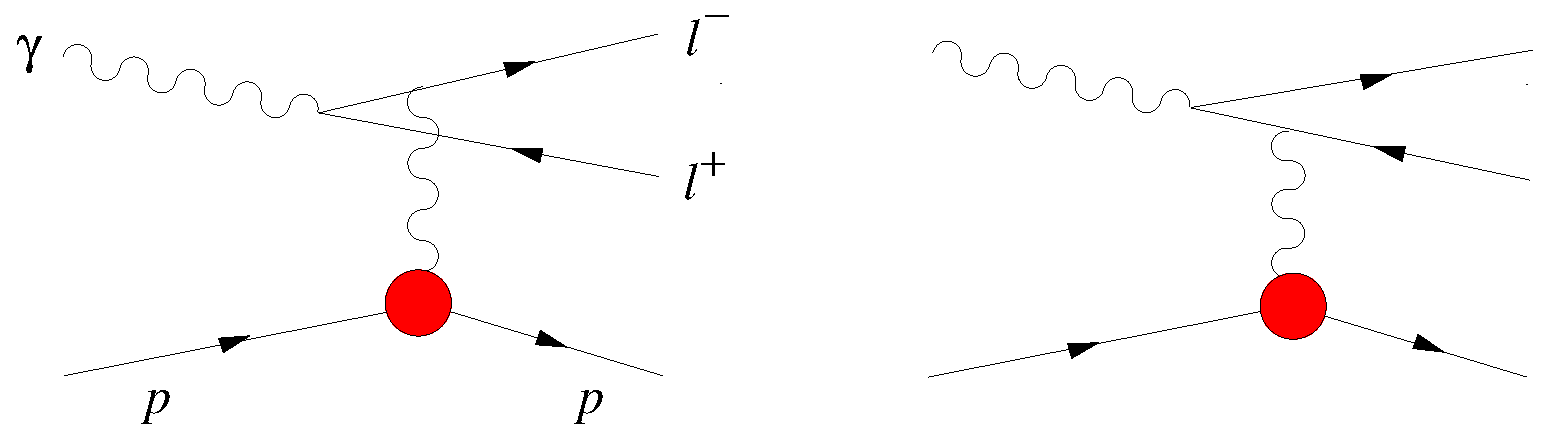
\includegraphics[scale=0.52]{BH.eps}
\caption{\small{The Feynman graphs for the Bethe-Heitler contribution to the 
$\gamma p \to l^+ l^- p$ process.}}
\label{fig:BH}
\end{center}
\end{figure}


\subsection{Leading-twist formalism}
\label{subsec:leading_twist}

To ensure the applicability of the leading twist formalism to the
$\gamma p \to l^{+} l^{-}p$ process (the left panel of
Fig.~\ref{fig:TCS_sketch}, one requires that 
(i) the timelike virtuality of the final-state photon, $Q^{\prime 2}$,
is sufficiently large to provide a hard scale,
(ii) the invariant photon-proton c.m. energy, $\sqrt{s}$, is sufficiently
large to ensure the usual DIS kinematics, and
(iii) the invariant momentum transfer squared $t$ is low, \textit{i.e.},
$|t| \leq 1$ GeV$^2$. 
The timelike nature of the final state also makes interpretation complicated
in the presence of resonances in the invariant mass of the produced lepton
pair. Hence, as shown in Fig.~\ref{fig:ee_to_hadrons}, an ideal mass range for
this experiment is $M_{\rho^\prime} < M_{l^{+} l^{-}} < M_{J/\psi}$, which
coincides well with JLab 12 GeV kinematics.
Since the invariant mass of the lepton pair, $M_{l^{+} l^{-}}$, is also the
timelike virtuality of the outgoing photon, $Q^\prime$, focusing on the
resonance-free region automatically satisfies condition (i) above.

The leading-twist formalism for TCS has been developed in Ref.
\cite{Berger:2001xd}. It is based on the factorization theorem
\cite{Collins:1998be} that allows one to express the TCS amplitude in
Eq.~(\ref{eq:TCS}) as convolutions of calculable hard-scattering kernels
with GPDs. The resulting quantities are called Compton form factors (CFFs).
One expects that as long as $Q^{\prime 2}$ is sufficiently large, the
leading-twist approximation (\textit{i.e.}, ignoring terms of the order
of $m_N^2/Q^{\prime 2}$, $m_l^2/Q^{\prime 2}$, and $|t|/Q^{\prime 2}$)
should work equally well for TCS as it does for DVCS. In other words,
one does not expect enhanced higher twist corrections specific to
TCS~\cite{Diehl:2003ny}.

To leading order in the strong coupling constant, $\alpha_s$, the TCS amplitude
is given by the two handbag diagrams presented in Fig.~\ref{fig:TCS_Handbag}.
To leading order in $\alpha_s$, the TCS amplitude is equivalent to the
DVCS amplitude, making it easier to test the universality of GPDs.
However, at the next-to-leading order, the expressions for the hard scattering
kernels for TCS and DVCS are different and, as a result, the TCS and DVCS CFFs
have different forms \cite{Pire:2011st,Pire:2012yq}. This is discussed further
in Sect.~\ref{subsec:NLO}.

The proton has four leading-twist parton-helicity non-flip quark GPDs. The
expressions for the corresponding CFFs, ${\cal H}_1$, ${\cal E}_1$,
${\tilde{\cal H}}_1$, and $\tilde{{\cal E}}_1$ are:
\begin{eqnarray}
{\cal H}_1(\eta,t) &= &\sum_q e_q^2 \int^{1}_{-1} \left(\frac{H^q (x,\eta,t)}{\eta-x+i \epsilon}
  -\frac{H^q (x,\eta,t)}{\eta+x+i \epsilon}\right) \,, \nonumber\\
{\cal E}_1(\eta,t) &= &\sum_q e_q^2 \int^{1}_{-1} \left(\frac{E^q (x,\eta,t)}{\eta-x+i \epsilon}
  -\frac{H^q (x,\eta,t)}{\eta+x+i \epsilon}\right) \,, \nonumber\\
\tilde{{\cal H}}_1(\eta,t) &= &\sum_q e_q^2 \int^{1}_{-1} \left(\frac{\tilde{H}^q (x,\eta,t)}{\eta-x+i \epsilon} +\frac{\tilde{H}^q (x,\eta,t)}{\eta+x+i \epsilon}\right) \,, \nonumber\\
\tilde{{\cal E}}_1(\eta,t) &= &\sum_q e_q^2 \int^{1}_{-1} \left(\frac{\tilde{E}^q (x,\eta,t)}{\eta-x+i \epsilon} +\frac{\tilde{E}^q (x,\eta,t)}{\eta+x+i \epsilon}\right) \,,
\label{eq:CFF_H1}
\end{eqnarray}
where the superscript $q$ denotes the quark flavor and $e_q$ the quark charge.
For brevity, we suppressed the $Q^2$-dependence of the GPDs and CFFs.
In Eq.~(\ref{eq:CFF_H1}), the light-cone fraction $\eta$, which in TCS plays
the role of the skewness $\xi$ in DVCS, is fixed by the external kinematics:
\begin{equation}
\eta=-\frac{(q-q^{\prime}) \cdot (q+q^{\prime})}{(p+p^{\prime}) \cdot (q+q^{\prime})} \approx \frac{Q^{\prime 2}}{2(s-M^2)-Q^{\prime 2}+t} \,.
\label{eq:eta}
\end{equation} 

\begin{figure}[t]
\begin{center}
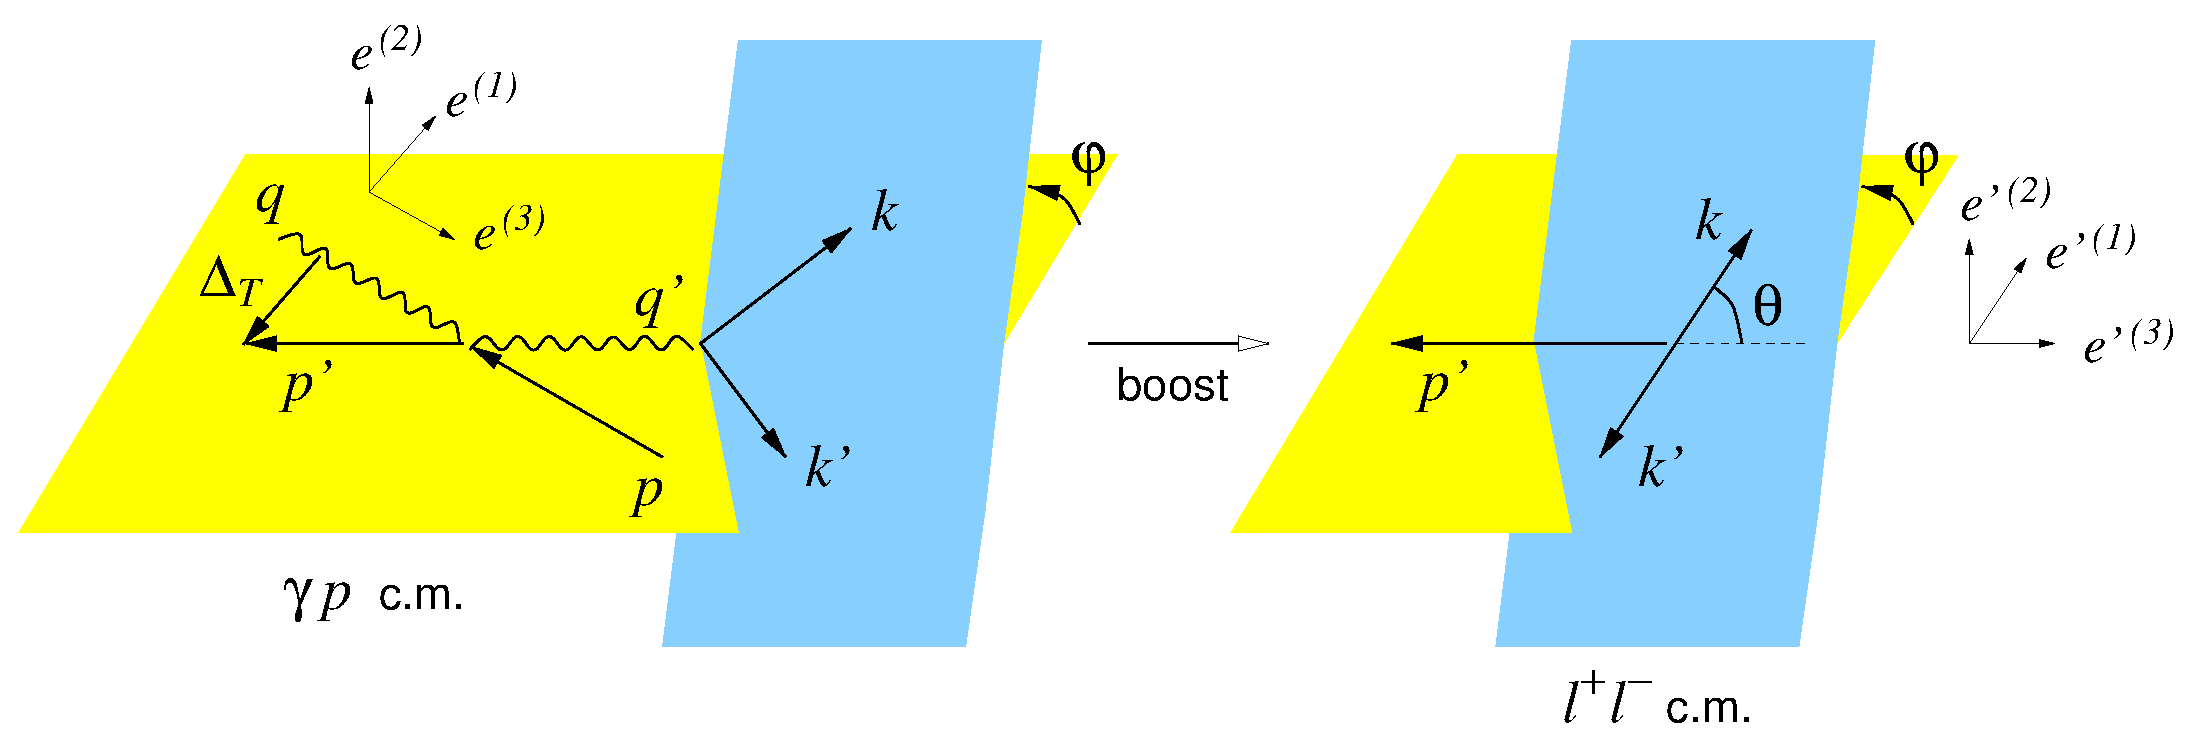
\includegraphics[scale=0.4]{Angle.eps}
\caption{\small{Momenta and angles involved in the TCS cross section in the
$\gamma p$ and $l^{+} l^{-}$ center-of-mass frames. Adopted from
\cite{Berger:2001xd}. Note that the angles $\varphi$ and $\theta$ will be
referred to explicitly as $\varphi_{CM}$ and $\theta_{CM}$ outside of the
motivation section to avoid confusion with the angles in the lab system.}}
\label{fig:Angle}
\end{center}
\end{figure}

From Eq.~(\ref{eq:CFF_H1}) it follows that the imaginary part of the CFFs can
be expressed in terms of GPDs along the so-called cross-over line,
\textit{i.e.}, at $x=\eta$ for quarks and $x=-\eta$ for antiquarks. The real
part of the CFFs is, on the other hand, sensitive to GPDs over the entire range
of $x$. For instance, the real part of the CFF ${\cal H}_1$ is given by:
\begin{equation}
\Re e {\cal H}_1(\eta,t) = \sum_q e_q^2 \, p.v.\int^{1}_{-1} \left(\frac{H^q (x,\eta,t)}{\eta-x}
  -\frac{H^q (x,\eta,t)}{\eta+x}\right) \,,
\label{eq:ReH1}
\end{equation}
where $p.v.$ stands for the principal value. The straightforward access to
the real part of CFFs (see Sect.~\ref{subsec:observables}) gives TCS
measurements the potential to constrain GPDs away from the cross-over line
in a wide range of $x$ and $\eta$.

\begin{figure}[t]
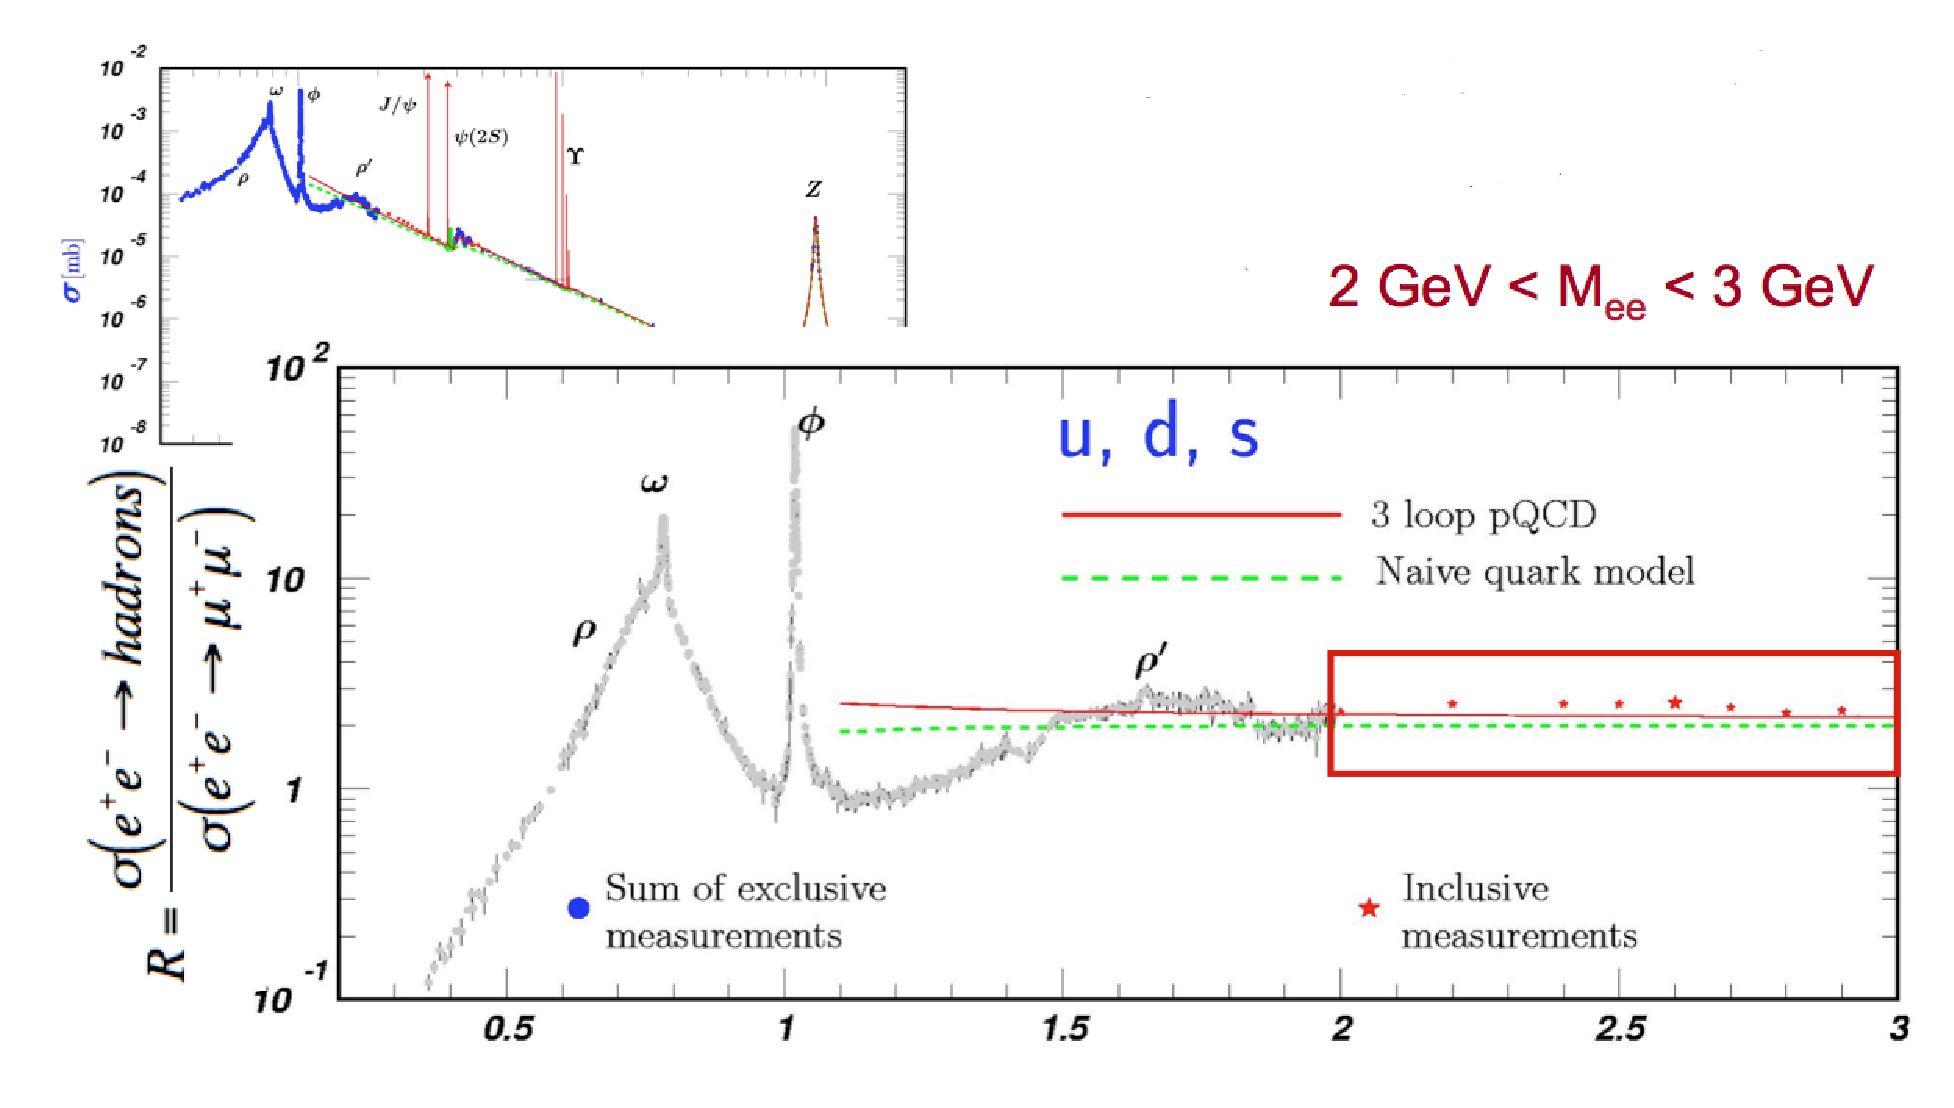
\includegraphics[width=125mm]{ee_to_hadrons.eps}
\caption{\small{Measurements of $e^+e^-$ annihilation into hadrons show a
resonance-free window between the $\rho'$ and the $J/\psi$, which is ideal
for TCS studies at 12 GeV.}}
\label{fig:ee_to_hadrons}
\end{figure}

The imaginary part of the Compton amplitude is now relatively well understood,
primarily through measurements of DVCS -- see, \textit{e.g.},
\cite{Guidal:2013rya}. However, much less is known about
the real part, which may become important at larger values of $x$, coinciding
with JLab 12 GeV kinematics.
The limited knowledge of the real part of the amplitude is reflected in GPD
model predictions, which are in good general agreement for the imaginary part,
but differ significantly when it comes to the real one. This is illustrated
in Figs.~\ref{fig:ReImH_tau} and \ref{fig:ReImH_t}, which show the real and
imaginary parts of the GPD $H$ as a function of $x$ and $-t$, respectively,
for two GPD models: the dual parametrization
\cite{Polyakov:2002wz,Guzey:2006xi,Guzey:2008ys,Polyakov:2008aa} and the
double distribution~\cite{Radyushkin:1998es}.
The potential of TCS to provide additional constraints on the real part
of CFFs is thus important for developing more accurate GPD models. The
TCS data could also be used in global fits of CFFs and for dispersion
relation analysis. This is discussed in more detail in
Sect.~\ref{subsec:amplitude_analysis} and
Sect.~\ref{subsec:dispersion}, respectively.

In TCS, the use of a circularly polarized photons allows to determinate
both the real and imaginary parts of the helicity amplitudes or CFFs
with comparable uncertainties. In contrast, DVCS measurements strongly
favor the imaginary part. The real part is only available through direct
cross section measurements or comparisons of cross sections measured
with electron and positron beams, both of which are significantly more
challenging than, for instance, the measurement of beam spin asymmetries
that give access to the imaginary part.

\begin{figure}[t]
\begin{center}
\includegraphics[scale=0.8]{TCS_Handbag.epsi}
\caption{\small{The handbag diagrams for TCS. The plus-momentum fractions
refer to the average proton momentum $(p+p^{\prime})/2$.}}
\label{fig:TCS_Handbag}
\end{center}
\end{figure}

In addition to discriminating between GPD models and constraining fits of
CFFs, a measurement of TCS may also offer a unique possibility to address
the issue of the so-called $D$-term~\cite{Polyakov:1999gs}.
Technically, the $D$-term is defined as the contribution to the GPD $H$ and
$E$ that provides the highest power of $\xi$ in Mellin moments of this GPD.
The $D$-term of the GPD $E$ has the same magnitude but opposite sign.
The $D$-term contribution to GPDs has support only in the region
$x \in [-\eta,\eta]$, which makes it elusive and inaccessible in the forward
limit. This unambiguously indicates that the $D$-term cannot be interpreted
in terms of the usual parton densities. Instead, the $D$-term describes the
emission of a $q {\bar q}$ pair by the nucleon, revealing the complex nature 
of the nucleon as a many-body system.

The $D$-term~\cite{Polyakov:1999gs} was originally introduced in
the context of the double distribution (DD) parametrization of GPDs
\cite{Radyushkin:1998es}, as an additional function required to generate the 
highest $n+1$ power of $xi$ in the $x^n$ moment of the GPD $H(x, xi)$. It was
realized \cite{Belitsky:2000vk} that the s]ame result could be achieved within
a single-DD parameterization (\textit{i.e.}, one using only the forward parton
distributions as input), but at the price of introducing singular expressions
requiring additional prescriptions. Because of the need to deal with singular
functions this method was not widely used for modeling GPDs. However, a
recent theoretical analysis of the single-DD parametrization
\cite{Radyushkin:2011dh} demonstrated explicity how all arising singular
expressions can be regularized and how the $D$-term naturally appears in
this approach, so that the relation between the two parametrizations is now
well understood. Coupled with the imbedded Regge formalism, the single-DD 
parametrization thus offers a new alternative approach to modeling GPDs.

The distribution of energy, momentum, and angular momentum in the nucleon
is characterized by form factors of the QCD energy-momentum tensor between
the nucleon states~\cite{Ji:1996ek,Jaffe:1989jz}, all of which can be
expressed in terms of GPDs. The $D$-term gives rise to one of these form
factors (denoted $C(t)$ or $d_1(t)$ in the literature).

It has been shown that in the Breit frame, this form factor can
be interpreted as describing the distribution of pressure and shear forces
acting on quarks inside the nucleon~\cite{Polyakov:2002yz}. Studies in
field-theoretical models show that the negative sign of the $D$-term is a
consequence of the stability of the nucleon~\cite{Goeke:2007fp}. This is
illustrated in Fig.~\ref{fig:D_term}, where the pressure $p(r)$ experienced
by quarks inside the nucleon is given as a function of the distance from the
center, $r$. Stability arises as a balance between repulsive forces in the
inner region, and attractive forces at large $r$, such that the stability
condition $\int_0^\infty {\rm d}r\,r^2p(r)=0$ holds.
The $D$-term is given by $d_1=5\pi M \int_0^\infty{\rm d}r\,r^4p(r)$ and the
additional weight $r^2$ in the integrand emphasizes the role of large
distances and binding forces inside the nucleon, leading to a negative
value of the $D$-term~\cite{Goeke:2007fp}.

Form factors of the QCD energy-momentum tensor can also be calculated from
first principles in lattice QCD. The QCDSF collaboration calculated the
$D$-term form factor $d_1(t)$ as a function of $-t$ for the pion
mass $m_{\pi}=640$ MeV~\cite{Gockeler:2003jfa}. The predictions of the chiral
quark-soliton model~\cite{Goeke:2007fp} used for the calculation shown in
Fig.~\ref{fig:D_term} are in agreement with the lattice data.

\begin{figure}[t]
\begin{center}
\includegraphics[scale=1.5]{comp_DD_Dual_Q2_5.eps}
\end{center}
\caption{\small{Imaginary (left) and real (right) parts of the GPD $H$
plotted as a function of $\tau = Q^{\prime 2} / (s - M^2)$, which is the
TCS equivalent of Bjorken $x$, for $Q^{\prime 2} = 5$ GeV$^2$ and $t = 0$.
The curves correspond to GPD models based on the dual parametrization
\cite{Polyakov:2002wz,Guzey:2006xi,Guzey:2008ys,Polyakov:2008aa} and the
double distribution~\cite{Radyushkin:1998es}, respectively.}}
\label{fig:ReImH_tau}
\end{figure}

The notion of the $D$-term is
%fundamental to two-photon processes, and is also
important for phenomenology because it
(i) is an integral ingredient of GPD modeling (see the discussion above),
(ii) gives an energy-independent ($\eta$-independent) contribution to
$\Re e H_1$ and $\Re e E_1$, and 
(iii) determines the subtraction constant in the dispersion relation
connecting the real and imaginary parts of the TCS and DVCS amplitudes
\cite{Radyushkin:2011dh,Anikin:2007yh,Diehl:2007jb,Polyakov:2007rv}.
In the language of Regge theory
\cite{Brodsky:1971zh,Brodsky:1972vv,Brodsky:1973hm,Brodsky:2008qu},
the $D$-term can be interpreted as originating from the $t$-channel
exchange with $J=0$ (the so-called fixed pole).


\subsection{TCS cross section and interference between TCS and BH amplitudes}
\label{subsec:observables}

\begin{figure}[t]
\begin{center}
\includegraphics[scale=1.5]{comp_DD_Dual_tdep_Q2_5.eps}
\end{center}
\caption{\small{Imaginary (left) and real (right) parts of the GPD $H$
plotted as a function of $-t$ for $Q^{\prime 2} = 5$ GeV$^2$ and
$\eta = 0.2$ (\textit{i.e.}, $\tau = 0.33$), where $\eta$ is the TCS
equivalent of $\xi$ in DVCS. The curves show the same models as in
Fig.~\ref{fig:ReImH_tau}.}}
\label{fig:ReImH_t}
\end{figure}

In the leading-twist approximation, the TCS cross section has
the following form~\cite{Berger:2001xd}:
\begin{equation}
\frac{d \sigma_{\rm TCS}}{dQ^{\prime 2} \,dt\, d cos \theta \, d \varphi} \approx \frac{\alpha^3_{\rm em}}{ 8 \pi s^2} \frac{1}{Q^{\prime 2}} \frac{1+\cos^2 \theta}{4} \sum_{\lambda,\lambda^{\prime}}
|M^{\lambda^{\prime}-,\lambda-}|^2 \,,
\label{eq:sigma_tcs}
\end{equation}
where $\alpha_{\rm em}$ is the fine structure constant and
$M^{\lambda^{\prime}-,\lambda-}$ are helicity amplitudes, with $\lambda$
($\lambda^{\prime}$) denoting the helicity of the incoming (outgoing) photon.
The TCS amplitude squared entering Eq.~(\ref{eq:sigma_tcs}) is expressed in
terms of the Compton form factors:
\begin{align}
\frac{1}{2}\sum_{\lambda,\lambda^{\prime}}|M^{\lambda^{\prime}-,\lambda-}|^2
&=(1-\eta^2)(|{\cal H}_1|^2+|\tilde{{\cal H}}_1|^2)-2 \eta^2 Re ({\cal H}_1^{\ast} {\cal E}_1+\tilde{{\cal H}}_1^{\ast} \tilde{{\cal E}}_1) 
\nonumber\\
&-(\eta^2+\frac{t}{4 m_N^2}) |{\cal E}_1|^2-\eta^2 \frac{t}{4 m_N^2} 
|\tilde{{\cal E}}_1|^2 \,.
\label{eq:m_tcs}
\end{align}

Theoretical analyses~\cite{Berger:2001xd,Pire:2008ea} have shown that the
TCS cross section is smaller than the BH cross section for JLab 12 GeV
kinematics, but like in DVCS, the BH and TCS amplitudes also interfere.
When the initial-state photon is unpolarized,
the interference term can be expressed as:
\begin{eqnarray}
 \frac{d\sigma_{\rm INT}}{dQ^{\prime 2}\, dt\, d(\cos\theta)\, d\varphi}
&=& {}- \frac{\alpha^3_{\rm em}}{4\pi s^2}\, \frac{1}{-t}\, \frac{M}{Q^{\prime}}\,
 \frac{1}{\tau \sqrt{1-\tau}}\, \frac{L_0}{L}
 \nonumber \\
&& {}\times\, \Big[\, \cos\varphi\, \frac{1+\cos^2\theta}{\sin\theta}\, \Re e \tilde{M}^{--}
   - \cos2\varphi\, \sqrt{2}\cos\theta\, \Re e \tilde{M}^{0-}
 \nonumber \\
&& {}+\, \cos3\varphi\, \sin\theta\, \Re e \tilde{M}^{+-}
   {}+\, {\cal O}\Big( \frac{1}{Q^{\prime}} \Big) \Big] \,,
\label{eq:interference}
\end{eqnarray}
where $M$ is the proton mass. The variable $\tau$,
\begin{equation}
\tau=\frac{Q^{\prime 2}}{2 (p \cdot q)}=\frac{Q^{\prime 2}}{s-M^2} \,,
\label{eq:tau}
\end{equation}
in TCS is the analog of the Bjorken variable $x_B=Q^2/(2 p \cdot q)$ in DVCS. 
To leading twist accuracy,
\begin{equation}
\eta=\frac{\tau}{2-\tau} \,,
\end{equation}   
where $\eta$ is given by Eq.~(\ref{eq:eta}).
In Eq.~(\ref{eq:interference}), $L_0$ and $L$ originate from the product of
final-state lepton propagators~\cite{Berger:2001xd} and
$\tilde{M}^{\mu^{\prime} \mu}$ are interference helicity amplitudes, where
$\mu$ ($\mu^{\prime}$) denotes the helicity of the incoming (outgoing) photon.
%While $\tilde{M}^{--}$ is a leading twist amplitude, $\tilde{M}^{0-}$ and 
%$\tilde{M}^{+-}$ are higher twist amplitudes.
In the handbag approximation, the photon (parton) helicity is conserved and,
as a result, the only surviving contribution in Eq.~(\ref{eq:interference})
comes from $\tilde{M}^{--}$:
\begin{equation}
\tilde{M}^{--}=\frac{2 \sqrt{t_0-t}}{M} \frac{1-\eta}{1+\eta} \Big[F_1 {\cal H}_1
-\eta(F_1+F_2)\tilde{{\cal H}}_1-\frac{t}{4 M^2} F_2 {\cal E}_1 \Big] \,,
\label{eq:M}
\end{equation}
where $-t_0=4 \eta^2 M^2/(1-\eta^2)$ is the minimal momentum transfer at a
given $\eta$ (modulo $1/Q^{\prime 2}$ corrections), and $F_1$ and $F_2$ are
the Dirac and Pauli elastic form factors of the proton, respectively.

\begin{figure}[t]
\begin{center}
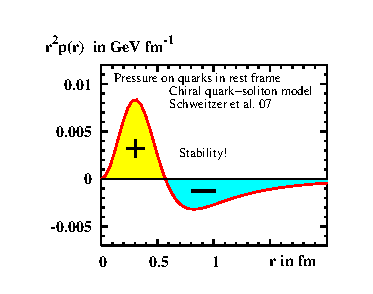
\includegraphics[scale=1.4]{pressure.eps}
\end{center}
\caption{\small{Pressure experienced by quarks inside the nucleon calculated
in the framework of the chiral quark-soliton model~\cite{Goeke:2007fp}.}}
\label{fig:D_term}
\end{figure}

Unpolarized photons (from a helicity-averaged electron beam) give access
to the real part of the CFFs. With a longitudinally polarized electron beam,
producing circularly polarized photons with polarization $\nu \neq 0$, one
can simultaneously study both the real and imaginary parts of the helicity
amplitudes using the full expression for the interference
term~\cite{Berger:2001xd}:
 \begin{eqnarray}
 \frac{d\sigma_{\rm INT}}{dQ^{\prime 2}\, dt\, d(\cos\theta)\, d\varphi}
&=& {}- \frac{\alpha^3_{em}}{4\pi s^2}\, \frac{1}{-t}\, \frac{M}{Q^{\prime}}\,
 \frac{1}{\tau \sqrt{1-\tau}}\, \frac{L_0}{L}
 \nonumber \\
&& {}\times\, \Big(\,\Big[\, \cos\varphi\, \frac{1+\cos^2\theta}{\sin\theta}\, \Re e\tilde{M}^{--}
   - \cos2\varphi\, \sqrt{2}\cos\theta\, \Re e \tilde{M}^{0-}
 \nonumber \\
&& {}+\, \cos3\varphi\, \sin\theta\, \Re e \tilde{M}^{+-}
   {}+\, {\cal O}\Big( \frac{1}{Q^{\prime}} \Big) \Big]
 \nonumber \\
&& {}+\, \nu\; \Big[\, \sin\varphi\, \frac{1+\cos^2\theta}{\sin\theta}\, \im\tilde{M}^{--}
   - \sin2\varphi\, \sqrt{2}\cos\theta\, \Im m\tilde{M}^{0-}
 \nonumber \\
&& {}+\, \sin3\varphi\, \sin\theta\, \im\tilde{M}^{+-} +\, {\cal O}\Big( \frac{1}{Q^{\prime}} \Big) \Big]\, \Big) \; ,
\label{eq:interference_2}
\end{eqnarray}
%Thus, measurements of TCS with polarized beams have the potential to
%constrain both the real and imaginary parts of the CFFs.

\begin{figure}[t]
\begin{center}
\includegraphics[scale=1.5]{R_DD_2012_E78.eps}
\end{center}
\caption{\small{
Predictions for the cosine moment of the weighted cross section shown as a
function of $-t$ at a fixed initial-state photon energy $E_\gamma = 7.8$ GeV
and $Q^{\prime 2} = 5$ GeV$^2$. 
The curves correspond to GPD models based on the dual parametrization
\cite{Polyakov:2002wz,Guzey:2006xi,Guzey:2008ys,Polyakov:2008aa} (blue)
and the double distribution~\cite{Radyushkin:1998es} (red), respectively.
The three lower (red) curves correspond to different strengths of the
$D$-term quantified by the parameter $\kappa$ in Eq.~(\ref{eq:dd1}).
The moment $R$, defined in Eq.~(\ref{eq:R}), is shown in the left panel,
while the right panel shows the corresponding curves for $R'$. The latter
is integrated over the $\theta$-$\varphi$ acceptance of the detector.
The details are explained in Sect.~\ref{sec:rates}. It is interesting to
note the while the different integration contour changes the absolute value of
$R'$ compared with $R$, it does not diminish the sensitivity.}}
\label{fig:r_theory}
\end{figure}

Under charge conjugation of the final-state lepton pair, which corresponds to
the transformation $\varphi \to \varphi + \pi$, the TCS and BH cross sections
are even, while the interference term is odd. This makes it possible to
project out the TCS-BH interference through the weighted and
$\theta$-integrated cross
section~\cite{Berger:2001xd}:
\begin{equation}
 \frac{dS}{dQ^{\prime 2}\, dt\, d\varphi} = 
  \int_{\pi/4}^{3\pi/4} d\theta\;
  \frac{L(\theta,\varphi)}{L_0(\theta)}\,
  \frac{d\sigma}{dQ^{\prime 2}\, dt\, d\theta\,d\varphi} \,.
%  \sum_{n=0}^\infty a_n\, \cos(n\varphi) \,.
\label{eq:S}
\end{equation}
The contribution of, for instance, $\Re e\tilde{M}^{--}$, can now be obtained
by taking the $\cos \varphi$-moment of $S$~\cite{Berger:2001xd}:
\begin{equation}
 R = \frac{\displaystyle 2 \int_0^{2\pi} d\varphi\, \cos\varphi\, \frac{dS}{dQ^{\prime 2}\, dt\, d\varphi}}
          {\displaystyle \int_0^{2\pi} d\varphi\, \frac{dS}{dQ^{\prime 2}\, dt\, d\varphi}} \,.
\label{eq:R}
\end{equation}

An example of the calculation of $R$ as a function of $-t$ at a fixed
initial-state photon energy $E_{\gamma}=7.8$ GeV and $Q^{\prime 2} = 5$
GeV$^2$ is shown in the left panel of Fig.~\ref{fig:r_theory}.
%As in Fig.~\ref{fig:ReImH_t},
The curves show predictions of calculations
based on two GPD models: the dual parametrization
\cite{Polyakov:2002wz,Guzey:2006xi,Guzey:2008ys,Polyakov:2008aa} (upper curve)
and the double distribution~\cite{Radyushkin:1998es} (lower three curves).
The difference in the magnitude of $R$ is quite significant, as would be
expected given the difference in $\Re e H$ shown in Fig.~\ref{fig:ReImH_t}.
The three lower curves correspond to different strengths of the
$D$-term~\cite{Goeke:2001tz} in the double distribution, as quantified by the
parameter $\kappa$ in Eq.~(\ref{eq:dd1}).
It is interesting to note that for the standard value of $\kappa$, the double
distribution predicts a cancellation with the $D$-term resulting in a small
$\Re e H$ -- a feature absent in the dual parametrization.
The right panel in Fig.~\ref{fig:r_theory} shows the same calculations
performed within the $\theta$-$\varphi$ acceptance of the detector.
The details are explained in Sect.~\ref{sec:rates}.
In the calculations with the double distribution, for the GPD $H$ we used:
\begin{equation}
H^q(x,\eta,t)=\int^1_{-1} d\beta \int^{1-|\beta|}_{-1+|\beta|} d \alpha \delta(x-\beta-\alpha \eta) \pi(|\beta|,\alpha) q(\beta,t)+ \kappa \frac{1}{N_f}\Theta(\eta-|x|) D(x/\eta,t)
\,,
\label{eq:dd1}
\end{equation}
where $\pi(\beta,\alpha)$ is the profile function that determines the degree
of skewness, $q(\beta,t)$ is the off-diagonal quark parton distribution that
reduces to the usual parton distribution in the $t=0$ limit, $D(x/\eta,t)$ is
the $D$-term, and $N_f=3$ is the number of active quark flavors. Note that we
introduced the coefficient $\kappa$ in front of the $D$-term to vary the
strength of its contribution. For the $D$-term, we used the standard expansion
in terms of the Gegenbauer polynomials $C_n^{3/2}$: 
\begin{equation}
D(z,t=0)=-(1-z^2)(d_1\, C_1^{3/2}(z)+d_3\, C ^{3/2}(z)+d_5\, C ^{3/2}(z)) \,.
\label{eq:D_term}
\end{equation}
The magnitude of the coefficients $d_i$ in Eq.~(\ref{eq:D_term}) was estimated
in the chiral quark-soliton model at a low normalization scale
\cite{Petrov:1998kf}; QCD evolution to the needed values of $Q^{\prime 2}$
somewhat decreases the values of the coefficients~\cite{Diehl:2003ny}.
To test the sensitivity of $R$ the $D$-term, we varied the parameter $\kappa$.
The three curves in Fig.~\ref{fig:r_theory} correspond to $\kappa=0.5$ (lower
curve), $\kappa=1$ (standard magnitude of the $D$-term), and $\kappa=2$
(upper curve), respectively.


\subsection{NLO corrections}
\label{subsec:NLO}
Timelike Compton Scattering (TCS) shares many features with spacelike DVCS
and allows to access the same GPDs. The amplitudes of these two reactions are
related at Born order by a simple complex conjugation, but they significantly
differ at next to leading order (NLO) in the strong coupling constant
$\alpha_s$ \cite{Muller:2012yq}. In the recent paper \cite{Moutarde:2013qs}
it was shown that the Born amplitudes of DVCS and TCS processes get sizeable
$O(\alpha_s)$ corrections and, even at moderate energies, the gluonic
contributions are by no means negligible. We stress that the timelike and
spacelike cases are complementary and that their difference deserves much
special attention.


Including gluon coefficient function appearing first at NLO,
and NLO corrections to the quark coefficient functions
\cite{Ji:1997nk,Mankiewicz:1997bk,Belitsky:1999sg,Freund:2001rk,Pire:2011st}
entering the TCS amplitudes, modifies significantly the values of the timelike
Compton form factors. Results are shown for two GPD models based on Double
Distributions (DDs): the so-called Goloskokov-Kroll (or GK) model
\cite{Goloskokov:2005sd,Goloskokov:2006hr,Goloskokov:2007nt,Kroll:2012sm},
and a model based on the simple factorizing ansatz for the $t$-dependence
\cite{Berger:2001xd} with MSTW08 PDFs \cite{Martin:2009iq}. The consequence
of a Polyakov-Weiss $D$-term \cite{Polyakov:1999gs}, following
\cite{Berger:2001xd} and \cite{Diehl:2003ny} is explored with the use
of the parametrization obtained by a fit to the chiral soliton model
\cite{Kivel:2000fg}.


\subsubsection{The TCS amplitudes}
After proper renormalization, the full Compton scattering amplitude (for both
DVCS or TCS) reads in its factorized form (at factorization scale $\mu_F$)
\begin{eqnarray}
\mathcal{A}^{\mu\nu} &=& -g_T^{\mu\nu}\int_{-1}^1 dx 
\left[
\sum_q^{n_F} T^q(x) F^q(x)+T^g(x) F^g(x)
\right] \nonumber \\
&+& i\epsilon_T ^{\mu\nu}\int_{-1}^1 dx 
\left[
\sum_q^{n_F} \widetilde{T}^q(x) \widetilde{F}^q(x)+\widetilde{T}^g(x) \widetilde{F}^g(x)
\right] \,,
\label{eq:factorizedamplitude}
\end{eqnarray}
where we omitted the explicit skewness dependence.
The renormalized coefficient functions are given by
\begin{eqnarray}
T^q(x)&=& \left[ C_{0}^q(x) +C_1^q(x) +\ln\left(\frac{Q^2}{\mu^2_F}\right) \cdot C_{coll}^q(x)\right] - ( x \to -x )  \,,\nonumber\\
T^g(x) &=& \left[ C_1^g(x) +\ln\left(\frac{Q^2}{\mu^2_F}\right) \cdot C_{coll}^g(x)\right] +( x \to -x )\,,\nonumber\\
\widetilde{T}^q(x)&=& \left[
\widetilde{C}_{0}^q(x) +\widetilde{C}_1^q(x) +\ln\left(\frac{Q^2}{\mu^2_F}\right) \cdot \widetilde{C}_{coll}^q (x)\right]
+( x \to -x )
\,,\nonumber\\
\widetilde{T}^g(x) &=&   \left[
\widetilde{C}_1^g(x) +\ln\left(\frac{Q^2}{\mu^2_F}\right) \cdot \widetilde{C}_{coll}^g(x)\right] - ( x \to -x )\,.
\label{eq:ceofficients}
\end{eqnarray} 

The difference between the DVCS and the TCS cases is the consequence of
analyticity (in $Q^2$) which leads to the relation \cite{Muller:2012yq}:
%%%%%%%%%%%%%%%%%%%%%%%%%%%%%%%%%%%%%%%%%%%%%%%%%%%%%%%%%%%%%%%%%%%%%%%%%%%%%%%%
\begin{eqnarray}
^{TCS}T(x,\eta) = \pm \left(^{DVCS}T(x,\xi=\eta) +  i \pi C_{coll}(x,\xi = \eta)\right)^* \,,
\label{eq:TCSvsDVCS}
\end{eqnarray}
where $+$~$(-)$ sign corresponds to the vector (axial) case.
%%%%%%%%%%%%%%%%%%%%%%%%%%%%%%%%%%%%%%%%%%%%%%%%%%%%%%%%%%%%%%%%%%%%%%%%%%%%%%%%


%%%%%%%%%%%%%%%%%%%%%%%%%%%%

\subsubsection{Timelike Compton Form Factors}

%%%%%%%%%%%%%%%%%%%%%%%%%%%%%%%%%%%%%%%%%%%%%%%%%%%%%%%%%%%%%%%%%

The timelike Compton Form Factors (CFF) at NLO,
$\mathcal{H}$ and $\widetilde{\mathcal{H}}$, defined as
\begin{eqnarray}
\mathcal{H}(\eta,t) &=& + \int_{-1}^1 dx \,
\left(\sum_q T^q(x,\eta)H^q(x,\eta,t)
 + T^g(x,\eta)H^g(x,\eta,t)\right) \nonumber \\
\widetilde{\mathcal{H}}(\eta,t) &=& - \int_{-1}^1 dx \,
\left(\sum_q \widetilde T^q(x,\eta)\widetilde H^q(x,\eta,t) 
+\widetilde T^g(x,\eta)\widetilde H^g(x,\eta,t)\right),
\label{eq:CFF}
\end{eqnarray}
are the GPD dependent quantities which enter the amplitudes.
For TCS they are defined through relations such as \cite{Berger:2001xd} 
\begin{equation}
\mathcal{A}^{\mu\nu}(\eta,t) = - e^2 \frac{1}{(P+P')^+}\, \bar{u}(P^{\prime}) 
\left[\,
   g_T^{\mu\nu} \, \Big(
      {\mathcal{H}(\eta,t)} \, \gamma^+ +
      {\mathcal{E}(\eta,t)} \, \frac{i \sigma^{+\rho}\Delta_{\rho}}{2 M}
   \Big)
   +i\epsilon_T^{\mu\nu}\, \Big(
    {\widetilde{\mathcal{H}}(\eta,t)} \, \gamma^+\gamma_5 +
      {\widetilde{\mathcal{E}}(\eta,t)} \, \frac{\Delta^{+}\gamma_5}{2 M}
    \Big)
\,\right] u(P) \, .
\label{eq:amplCFF}
\end{equation}
We present our results for $Q^2 = \mu_F^2 = \mu_R^2 = 4 $ GeV$^2$,
and use the value $\alpha_S = 0.3$~.


%%%%%%%%%%%%%%%%%%%%%%%%%%%%%%%%%%%%%%%%%%%%%%%%%%%%%%%%%%%%%%%%%

%%%%%%%%%%%%%%%%%%%%%%%%%%%%%%%%%%%%%%%%%%%%%%%%%%%%%%%%%%%%%%%%%%%%%%%%
\begin{figure}[hp]
\begin{center}
  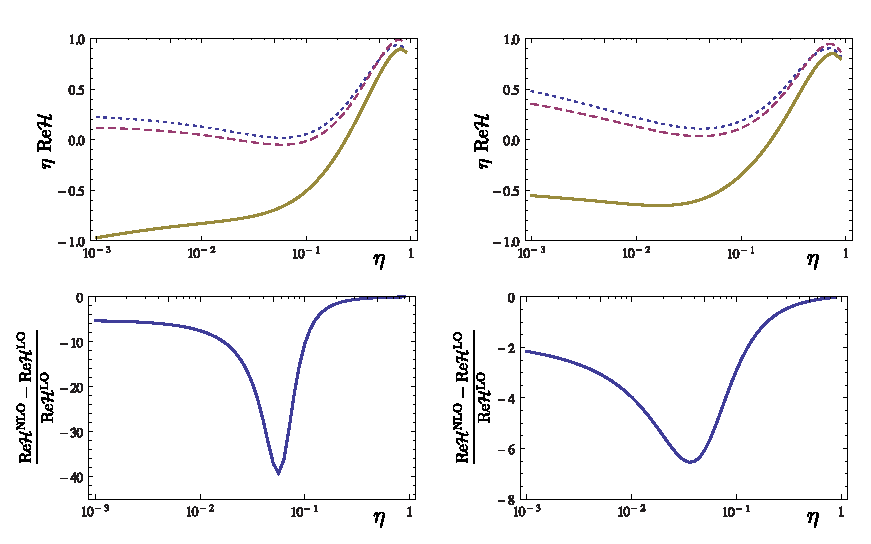
\includegraphics[width= 0.85\textwidth]{TCS_Re_2x2_nice.eps} 
\caption{The real part of the {\it timelike} Compton Form Factor
$\mathcal{H}$ multiplied by $\eta$, as a function of $\eta$ in the double
distribution model based on Goloskokov-Kroll (upper left) and MSTW08 (upper
right) parametrizations, for $\mu_F^2=Q^2=4$~GeV$^2$ and $t=-0.1$~GeV$^2$.
Below the ratios of the NLO correction to LO result of the corresponding
models.}
\label{fig:TCSRe2x2}
\end{center}
\end{figure}
%%%%%%%%%%%%%%%%%%%%%%%%%%%%%%%%%%%%%%%%%%%%%%%%%%%%%%%%%%%%%%%%%
%%%%%%%%%%%%%%%%%%%%%%%%%%%%%%%%%%%%%%%%%%%%%%%%%%%%%%%%%%%%%%%%%%%%%%%%
\begin{figure}[ht]
\begin{center}
  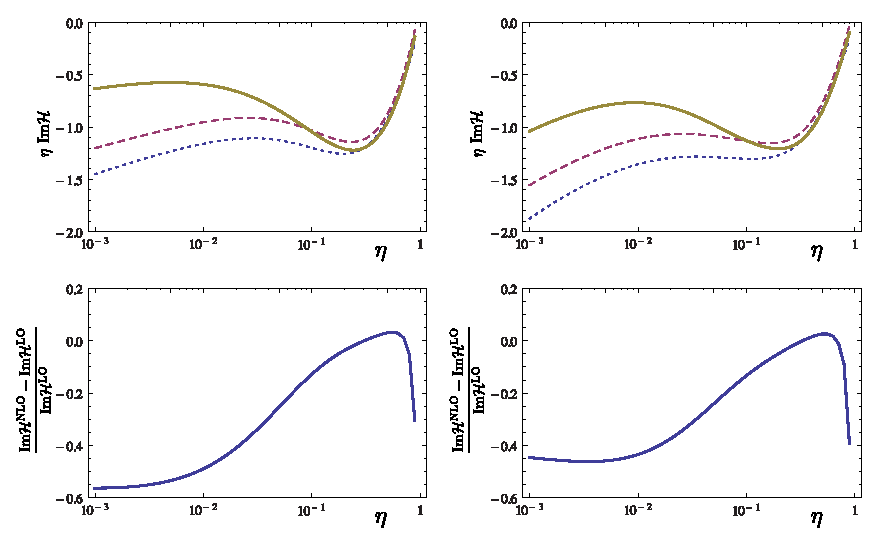
\includegraphics[width= 0.85\textwidth]{TCS_Im_2x2_nice.eps} 
\caption{The imaginary part of the {\it timelike} Compton Form Factor
$\mathcal{H}$ multiplied by $\eta$, as a function of $\eta$ in the double
distribution model based on Goloskokov-Kroll (upper left) and MSTW08 (upper
right) parametrizations, for $\mu_F^2=Q^2=4$~GeV$^2$ and $t=-0.1$~GeV$^2$.
Below the ratios of the NLO correction to LO result of the corresponding
models.}
\label{fig:TCSIm2x2}
\end{center}
\end{figure}
%%%%%%%%%%%%%%%%%%%%%%%%%%%%%%%%%%%%%%%%%%%%%%%%%%%%%%%%%%%%%%%%%
To show the importance of including NLO effects in the timelike CFFs relevant
to timelike Compton scattering, we plot in Fig.~\ref{fig:TCSRe2x2} and
Fig.~\ref{fig:TCSIm2x2}, the real and imaginary parts of the CFF $\mathcal{H}$
for the GK and the MSTW08 models of GPDs, for the invariant mass of the lepton
pair $Q'^2=4$ GeV$^2$, $t=-0.1$ GeV$^2$. For the imaginary part the correction
does not exceed $40\%$. In the real part, the correction is of the order of
few hundred percent. We observe that the main part of that large correction
comes from the contribution of gluonic GPDs. 

%\begin{figure}[ht]
%\begin{center}
%  \includegraphics[width=7cm]{ReHerr_nice.eps}  ~~~~ \includegraphics[width= 7cm]{ImHerr_nice.eps} 
%\caption{The real (left) and imaginary(right) parts of the TCS Compton Form Factor $\mathcal{H}$ multiplied by $\eta$, as a function of $\eta$ in the double distribution model based on MSTW08 parametrization, for $\mu_F^2=Q^2=4$~GeV$^2$ and $t= -0.1$~GeV$^2$. The dotted line shows the LO result and shaded bands around solid lines show the effect of a one sigma uncertainty of the input MSTW08 fit to the full NLO result.}
%\label{fig:TCSerror}
%\end{center}
%\end{figure}
%%%%%%%%%%%%%%%%%%%%%%%%%%%%%%%%%%%%%%%%%%%%%%%%%%%%%%%%%%%%%%%%%%%%


The $D$-term contribution to the CFF is a $\eta$-independent quantity and it
has both a real and an imaginary parts at NLO. 
We show in Tab.~\ref{tableDTCS} the values of this $D$-term contribution in
the LO and NLO cases. Its relative effect on the imaginary part of the CFF
decreases significantly when $\eta$ decreases, from 10 to 1 and 0.1\% when
$\eta$ decreases from 0.1 to 0.01 and to 0.001.
%Table
\begin{table*}[h]
\begin{center}
\begin{tabular}{|c||c|c|}
\hline
 & Re$\mathcal{H_D}$ &  Im$\mathcal{H_D}$ \\ \hline \hline
LO &  -2.59 & 0 \\ \hline
NLO quark contribution & -0.16 & -0.85 \\ \hline
NLO gluon contribution & 0.18 & 0.16 \\ \hline
Full NLO & -2.57 & -0.69 \\ 
\hline
\end{tabular}
\caption{\small Different contributions to the $D$-term. The values of the
real part coincides for spacelike and timelike CFF $\mathcal{H}$, while the
imaginary part is non-vanishing only for the timelike case.}
\label{tableDTCS}
\end{center}
\end{table*}

We then compare TCS and DVCS by plotting the ratio of NLO corrections on
Fig.~\ref{fig:TCStoDVCS}. There is a striking difference in the magnitude of
the corrections to the real part of CFFs, mostly insensitive to the choice of
GPD parametrizations. As discussed in Ref.~\cite{Muller:2012yq}, this is a
consequence of Eq.~(\ref{eq:TCSvsDVCS}) which by adding a phase to the
dominant imaginary part of the spacelike CFF at small skewness, gives rise
to a sizeable real part of the corresponding CFF in the timelike case.
Such large corrections to the real part of CFFs will have a significant
influence on observables which depend on the interference of the TCS process
with the Bethe-Heitler amplitude, {\sl i.e.} connected to the azimuthal
angular distribution of the leptons. 
\begin{figure}[ht]
\begin{center}
  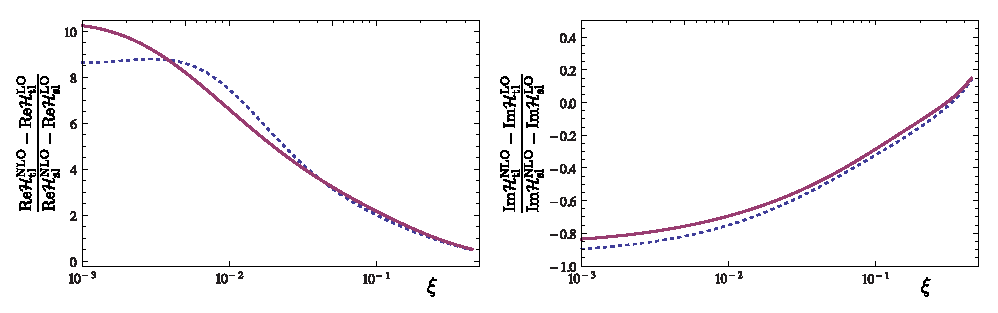
\includegraphics[width= 0.85\textwidth]{TCStoDVCS_1x2_nice.eps}
\caption{The ratio of the timelike to spacelike NLO corrections in the real
(left) and imaginary (right) part of the Compton Form Factor $\mathcal{H}$,
as a function of $\xi$ in the double distribution model based on the
Goloskokov-Kroll (dashed) and MSTW08 (solid) parametrizations, for
$\mu_F^2=Q^2=4$~GeV$^2$ and $t= -0.1$~GeV$^2$. For comparison timelike CFFs
where calculated at $\eta = \xi$.}
\label{fig:TCStoDVCS}
\end{center}
\end{figure}


\subsubsection{Cross sections and asymmetries}
Let us now pass to our estimates for the observables in TCS. Generally we
observe that the inclusion of the NLO corrections is more important at small
skewness. We also see that the Bethe-Heitler dominates the integrated
cross-section for this kinematics. In consequence, more differential
observables, as the azimuthal $\phi$ dependence (with angles $\theta$ and
$\phi$ defined in Ref.~\cite{Berger:2001xd}) reveal in a better way the
different contributions. Moreover simple $\phi$ dependence of the interference
term allows for an easy access to the real part of the CFFs which, as we
observed in Fig.~\ref{fig:TCSRe2x2}, is subject to big NLO corrections. We
indeed observe that effect on the Fig.~\ref{fig:xsec_phidep}, which shows the
$\phi$ dependence of the unpolarized differential cross sections for pure BH
process, and with a LO and NLO corrections to the interference term.
%
\begin{figure}[ht]
\begin{center}
%\epsfxsize=0.8\textwidth
 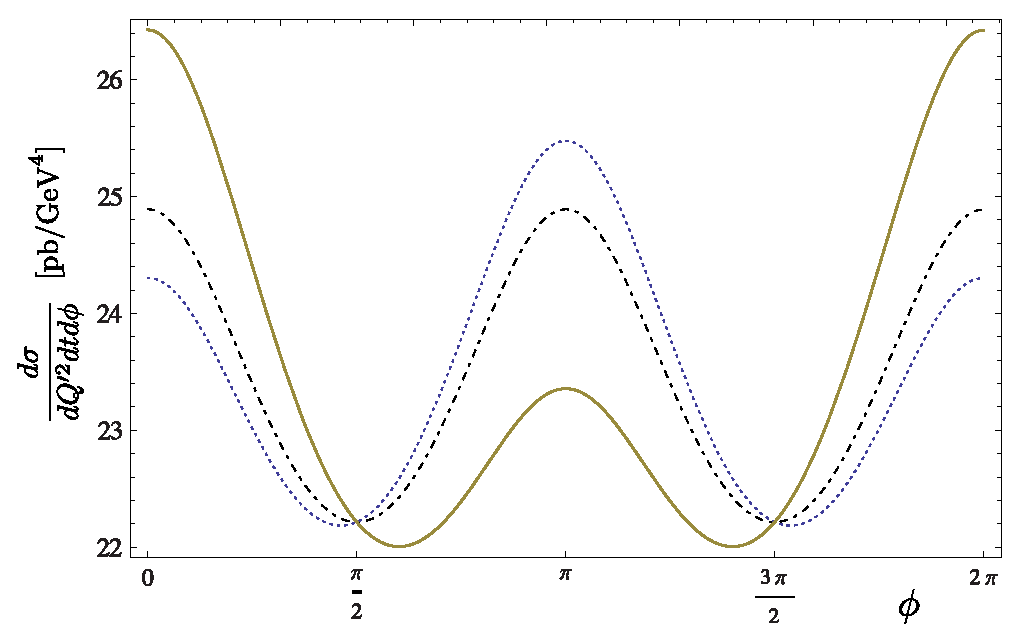
\includegraphics[width=8 cm]{xsec_phidep.eps}
\caption{The $\phi$ dependence of the cross-section at $E_\gamma = 10$ GeV,
 $Q^2 = \mu_F^2 = 4$~GeV$^2$, and $t= -0.1$~GeV$^2$ integrated over $\theta
\in (\pi/4,3\pi/4)$: pure Bethe-Heitler contribution (dash-dotted),
Bethe-Heitler plus interference contribution at LO (dotted) and NLO (solid).}
\label{fig:xsec_phidep}
\end{center}
\end{figure}

\begin{figure}[ht]
\begin{center}
%\epsfxsize=0.8\textwidth
  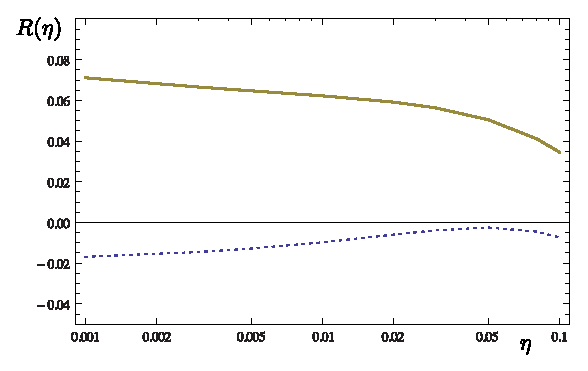
\includegraphics[width=8 cm]{R.eps}
\caption{Ratio R defined by Eq.~(\ref{eq:R_ratio}) as a function of $\eta$,
for $Q^2 = \mu_F^2 = 4$~GeV$^2$ and $t= -0.1$~GeV$^2$. The dotted line
represents LO contribution and the solid line represents NLO result.}
\label{fig:Ratio_R}
\end{center}
\end{figure}


%\begin{equation}
%\frac{
%\frac{d\sigma}{dQ'^2dtd\varphi}\left(\phi=0\right)
%-\frac{d\sigma}{dQ'^2dtd\varphi}\left(\phi=\pi\right)
%}
%{
%\frac{d\sigma_{BH}}{dQ'^2dtd\varphi}\left(\phi=0\right)
%}\,.
%\label{eq:Ratio_INT_BH_xi}
%\end{equation}

To quantify how big the deviation is from the pure Bethe-Heitler process in
the unpolarized cross section we calculate (see Fig.~\ref{fig:Ratio_R}) the
ratio R, defined in Ref.~\cite{Berger:2001xd} by
\begin{equation}
R(\eta) =  \frac{2\int_0^{2 \pi} d \varphi \,\cos \varphi\, \frac{dS}{dQ'^2dtd\varphi}}{\int_0^{2 \pi} d \varphi\frac{dS}{dQ'^2dtd\varphi}}
\,,
\label{eq:R_ratio}
\end{equation}
where $S$ is a weighted cross section given by Eq.~(43) of
Ref.~\cite{Berger:2001xd}.
It is plotted in Fig.~\ref{fig:Ratio_R} as a function of the skewness $\eta$
for $Q^2 = \mu^2 = 4$~GeV$^2$, and $t= -0.2$~GeV$^2$. In the leading twist the
numerator is linear in the real part of the CFFs, and the denominator, for the
kinematics we consider, is dominated by the Bethe - Heitler contribution. The
inclusion of NLO corrections to the TCS amplitude is indeed dramatic for such
an observable and includes also change of sign.

%This have a consequence also for the ratio $R$ defined by eq.\ref{Eq:DD}ref{RRatio}. That ratio calculated for the same kinematical region is equal on the leading order to $R_{LO} = -0.04 $ and on the next-to-leading $R_{NLO} = 0.06$.

%%%%%%%%%%%%%%%%%%%%%%%%%%%%%%%%%%%%%%%%%%%%%%%%%%%%%%%%%%%%%%%%%%%%%%%%


Imaginary parts of the CFFs are accessible through observables making use of
photon circular polarizations \cite{Berger:2001xd}. The photon beam circular
polarization asymmetry
\begin{equation}
A= \frac{\sigma^+ - \sigma^-}{\sigma^+ + \sigma^-}\,,
\end{equation}
is shown on the left part of Fig.~\ref{fig:Asymmetry_xi}, as a function of
$\phi$ for the kinematic variables relevant for JLab:
$Q^2 =4$~GeV$^2$= $\mu_F^2$, $t=-0.1$~GeV$^2$ and $E_\gamma = 10$~GeV (which
corresponds to $\eta \approx 0.11$). The same quantity is shown on the right
panel of Fig.~\ref{fig:Asymmetry_xi} as a function of $\eta$ for
$\phi = \pi/2$ and $Q^2 =4$~GeV$^2$= $\mu_F^2$. The effect of the NLO
corrections on that observable is rather large, around $10\%$ in the $\eta$
range most relevant for JLab kinematics.

\begin{figure}[ht]
\begin{center}
%\epsfxsize=0.8\textwidth
  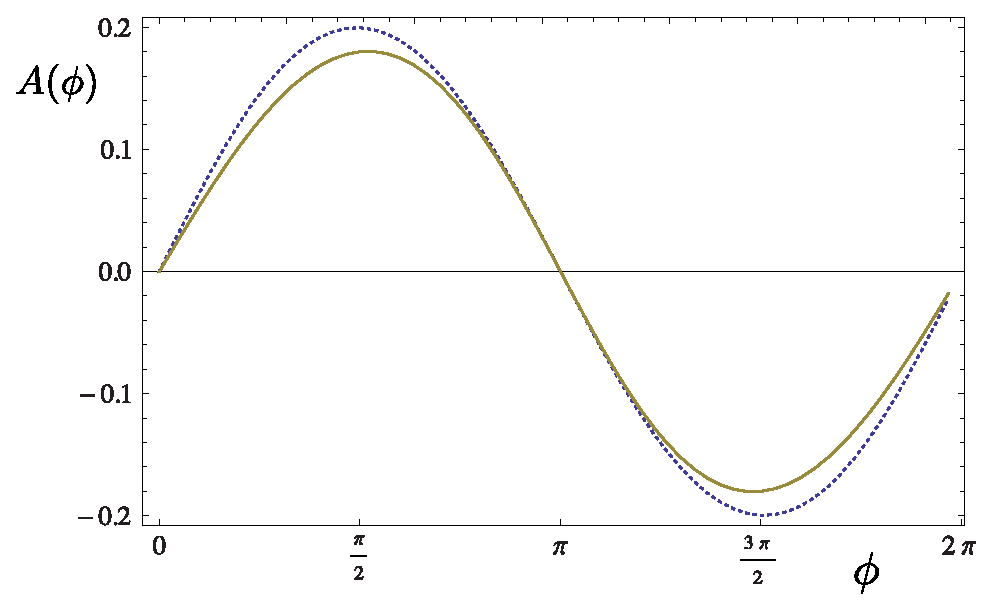
\includegraphics[width=0.4\textwidth]{Asymmetry_E_10_t_01_Q_2_nice.eps}
  \hspace{0.05\textwidth}
  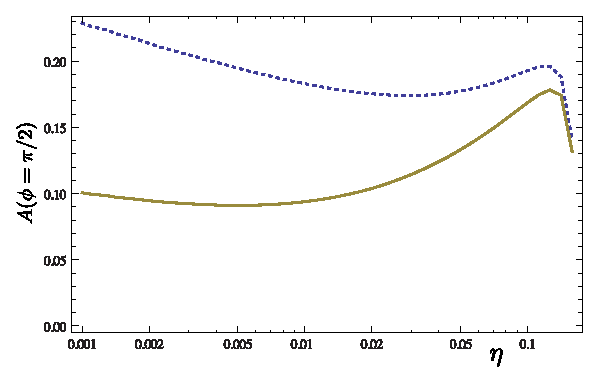
\includegraphics[width=0.4\textwidth]{Asymmetry_xi_nice.eps}
\caption{
(Left) Photon beam  circular polarization asymmetry as a function of $\phi$,
for $t=-0.1$~GeV$^2$, $Q^2 = \mu_F^2 = 4$~GeV$^2$, integrated over $\theta
\in (\pi/4,3\pi/4)$ and for $E_\gamma = 10$~GeV ($\eta \approx 0.11$).
(Right) The $\eta$ dependence of the photon beam circular polarization
asymmetry for $Q^2 = \mu_F^2 = 4$~GeV$^2$, and $t= -0.2$~GeV$^2$ integrated
over $\theta \in (\pi/4,3\pi/4)$. The LO result is shown as the dotted line,
the full NLO result by the solid line.}
\label{fig:Asymmetry_xi}
\end{center}
\end{figure}



\subsection{Amplitude analysis of Compton form factors}
\label{subsec:amplitude_analysis}
While the theory and phenomenology of exclusive processes and GPDs are now
rather mature, the extraction of GPDs (Compton form factors) from available
data is a complex problem that was started to be tackled only recently
\cite{Guidal:2008ie,Kumericki:2007sa,Moutarde:2009fg,Guidal:2009aa,
Guidal:2010ig,Guidal:2010de,Moutarde:2010uk,Moutarde:2011zz,Kumericki:2011aa}.
The complications include (i) generally low rates of exclusive processes, (ii)
the limited number of independent experimental observables which are measured,
(iii) the number of proton GPDs (at leading twist, the proton has four quark
and four gluon parton-helicity-conserving GPDs) which (iv) are themselves
functions of four variables, and (v) the fact that even at the leading order,
GPDs enter experimental observables in the form of convolutions with known
kernels. These convolutions are called Compton form factors (CFFs). There are
eight CFFs associated with the four quark helicity-conserving GPDs, namely
$Re\{\mathcal{H}\}$, $Re\{\mathcal{E}\}$, $Re\{\tilde{\mathcal{H}}\}$,
$Re\{\tilde{\mathcal{E}}\}$, $Im\{\mathcal{H}\}$, $Im\{\mathcal{E}\}$,
$Im\{\tilde{\mathcal{H}}\}$, and $Im\{\tilde{\mathcal{E}}\}$.

A quasi model-independent CFF fitting procedure of
Refs.~\cite{Guidal:2008ie,Guidal:2009aa,Guidal:2010ig,Guidal:2010de}
has been implemented for the TCS process. The procedure simultaneously fits
various experimental observables at a given kinematical point (\textit{i.e.},
$\eta$, $|t|$, and $Q^{\prime 2}$ for the TCS process), to the well-known
leading-twist and leading-order TCS and BH amplitude,

\begin{figure}[t]
\begin{center}
\mbox{
\subfigure{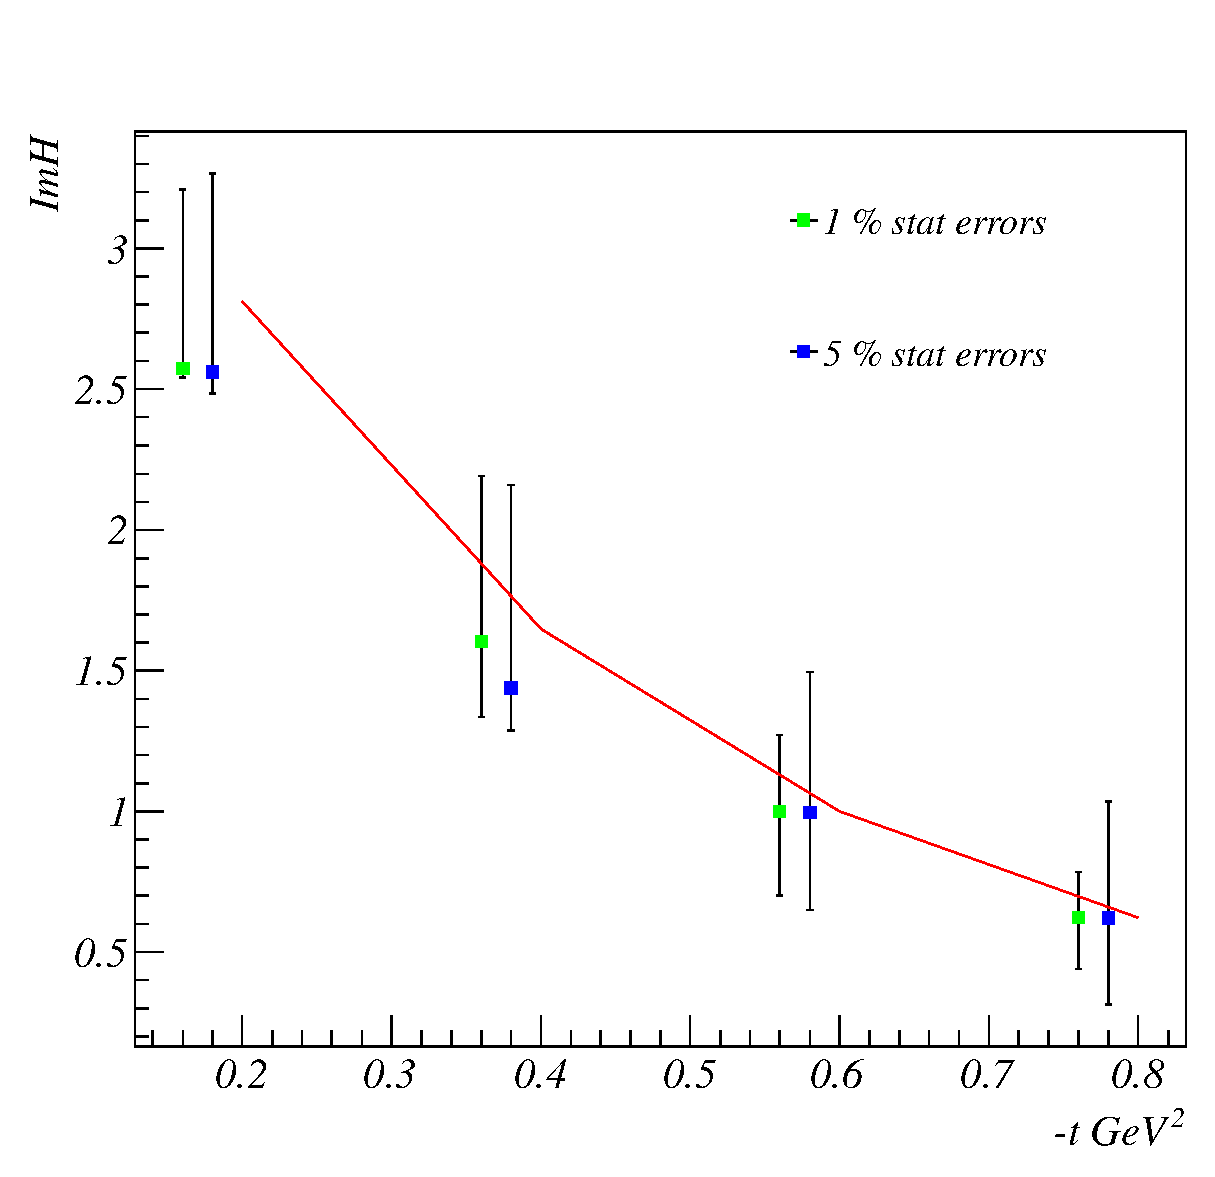
\includegraphics[scale=0.35]{ImH_theta.eps}} \quad
\subfigure{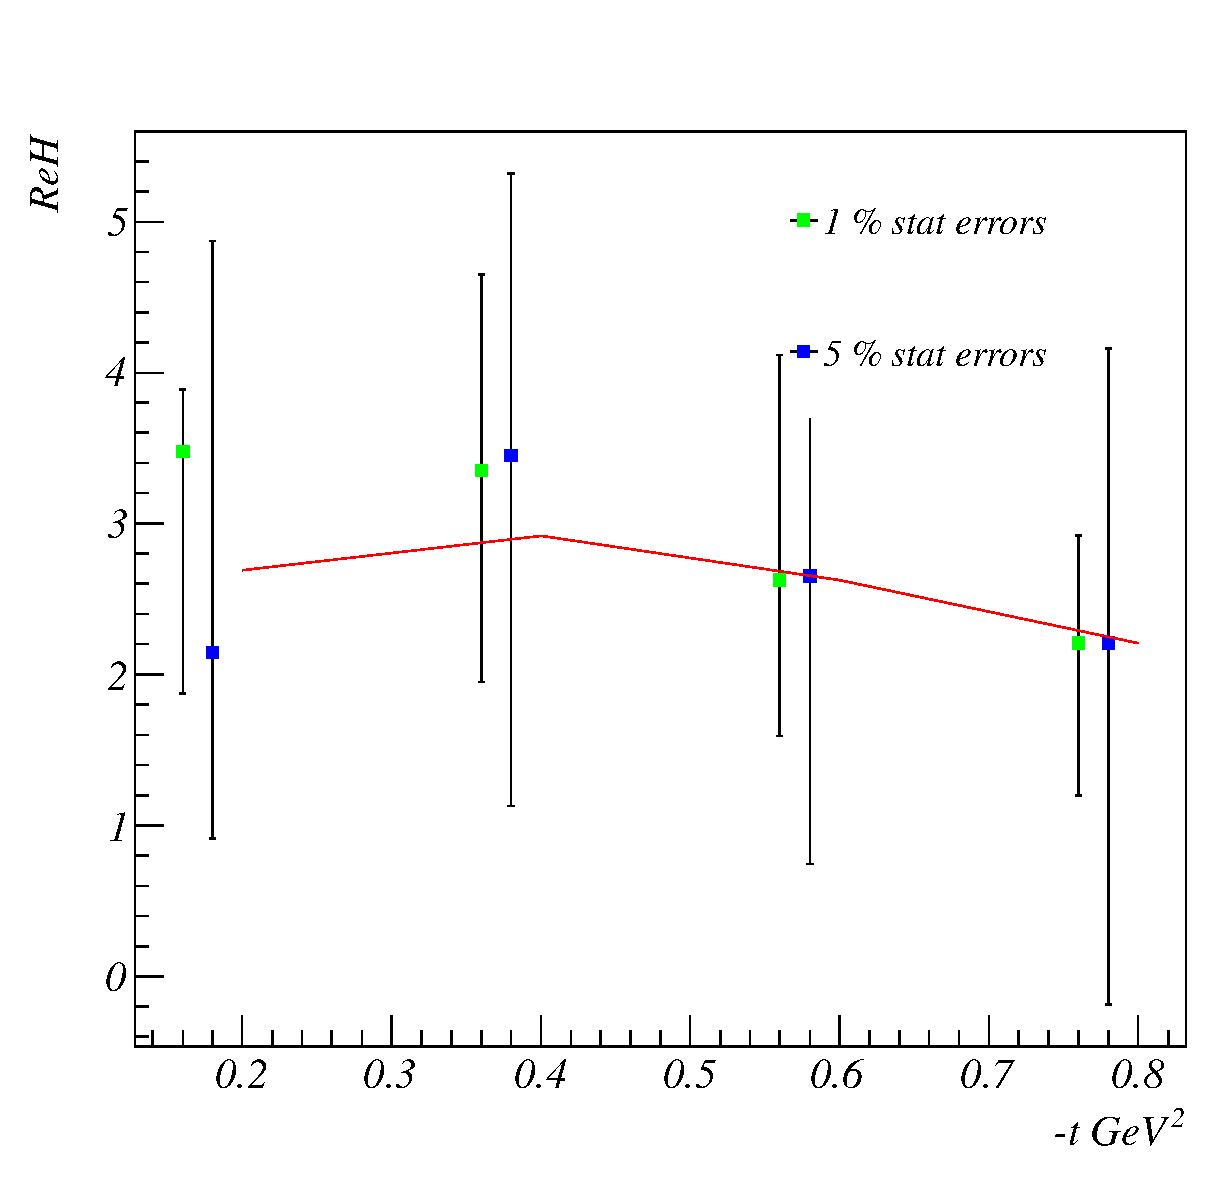
\includegraphics[scale=0.35]{ReH_theta.eps}}}
\end{center}
\caption{\small{
{\it Left panel:} result on the extraction of the $Im\{\mathcal{H}\}$ CFF 
for $E_e$=11 GeV, $Q'^2$=4 GeV$^2$ and $-t$=0.2, 0.4, 0.6 and 0.8 GeV$^2$.
{\it Right panel:} same for $Re\{\mathcal{H}\}$.
Symbols and curves are described in the text.}}
\label{fig:TCS_fits}
\end{figure}

This approach has been very successful for the DVCS process, allowing to
extract, at the $\approx$ 30\% level, from various beam- or target-polarized
observables, three CFFs
($Re\{\mathcal{H}\}$, $Im\{\mathcal{H}\}$, and $Im\{\tilde{\mathcal{H}}\}$)
in JLab and HERMES kinematics~\cite{Guidal:2010de}.
For this procedure to be efficient, it is important to simultaneously fit
several experimental observables. Fitting eight CFFs with only one observable
makes the problem too under-constrained.

To illustrate the quasi model-independent approach, we have generated
pseudo-data in typical 12 GeV kinematics ($E_e$=11 GeV, $Q'^2$=4 GeV$^2$,
and $|t|$=0.2, 0.4, 0.6, and 0.8 GeV$^2$), for two TCS observables that
we plan to extract: the unpolarized cross section and the polarized beam
asymmetry. The CFFs used for the generation of the data were the
VGG~\cite{Vanderhaeghen:1999xj,Guidal:2004nd} ones. Assuming different values
for the experimental uncertainties on these two observables, we then fitted
them and attempted to recover the generated CFFs. The results of the fit
revealed a sensitivity to four CFFs:
$Re\{\mathcal{H}\}$, $Im\{\mathcal{H}\}$, $Re\{\tilde{\mathcal{H}}\}$, and
$Im\{\tilde{\mathcal{H}}\}$. Fig.~\ref{fig:TCS_fits} shows our result for
$Re\{\mathcal{H}\}$ and $Im\{\mathcal{H}\}$, which are the most constrained.
The red curve shows the generated CFFs, while the blue and green points show
the resulting fitted CFFs with their associated error bar, corresponding to
a 5\% and a 1\% uncertainty, respectively, on the experimental cross section
and asymmetry. Due to systematics, a 1\% uncertainty on the experimental
observable will probably always be unrealistic, but we nevertheless show
the result for reference.
Fig.~\ref{fig:TCS_fits} shows that with a 5\% total experimental uncertainty,
we should be able to extract the $Re\{\mathcal{H}\}$ and $Im\{\mathcal{H}\}$
CFFs with $\approx$ 60\% and 20\% error, respectively.
The resulting errors may appear large, but we stress that firstly, this
fitting method aims to be model-independent, and secondly, that in this
procedure, the error on the extracted CFFs is not directly proportional to the
precision of the experimental data but rather reflects the influence (or our
ignorance) of all the other CFFs. The sub-dominant (kinematically suppressed)
CFFs enter the fitting procedure and have an impact on the error.
Therefore, the errors on $Re\{\mathcal{H}\}$ and $Im\{\mathcal{H}\}$ in
Fig.~\ref{fig:TCS_fits} reflect the ``correlation'' between all eight CFFs.
Increasing the number of experimental observables to be fitted (for instance,
using a longitudinally and/or a transversely polarized target) will strongly
reduce the fitting errors, and the uncertainties on the extracted CFFs will
more directly reflect the precision of the data. Alternatively, model
constraints can be added to achieve a similar result with only two
observables. Either way, ultimately data with small uncertainties, both
statistical and systematic, will have a large impact on our understanding of
the CFFs. But the initial results presented in Fig.~\ref{fig:TCS_fits} already
demonstrate the general feasibility of extraction of GPDs from TCS data.


\subsection{Comment on dispersion analysis}
\label{subsec:dispersion}

Dispersion relations provide a very powerful and model-independent method
to relate the real and imaginary parts of scattering amplitudes based on
such general properties as analyticity and crossing symmetry. For hard
exclusive reactions, dispersion relations have been established and analyzed
for DVCS, double DVCS (where the incoming photon has a spacelike virtuality
and the outgoing photon is timelike), and for exclusive meson
production~\cite{Anikin:2007yh,Diehl:2007jb,Polyakov:2007rv}.

For instance, for the CFF ${\cal H}^{q[+]}$ (the superscript $[+]$
indicates the singlet combination corresponding to $q+{\bar q}$), 
one obtains the dispersion relation~\cite{Diehl:2007jb}:
\begin{equation}
\Re e {\cal H}^{q[+]}(\xi)=\frac{1}{\pi} \int^{\infty}_{1} d\omega \Im m C^{q[+]}(\omega) \int^{1}_{-1}dx \Bigg\{H^q(x,\frac{x}{\omega})\Big[\frac{1}{\omega \xi -x}-\frac{1}{\omega \xi+x}\Big]+\frac{2 D^q(x)}{\omega-x} \Bigg\} \,,
\label{eq:DR}
\end{equation}
where $C^{q[+]}$ is the process-dependent hard-scattering kernel.
The $D$-term enters the dispersion relation as a subtraction constant,
\textit{i.e.}, it gives an energy-independent contribution to
$\Re e {\cal H}^{q[+]}$.
The importance of the dispersion relation in Eq.~(\ref{eq:DR}) 
is that it quantifies the amount of information on GPDs that can be 
extracted from the real and imaginary parts of CFFs or, more generally, 
from amplitudes of exclusive processes. In addition, it provides a
practical consistency check for models of GPDs.
While dispersion relations for the TCS amplitudes have not yet been worked
out, there should be no major difficulty in establishing them analogously
to the cases that have already been considered.
%The analytic structure of the TCS amplitude is
%richer than that of the DVCS amplitude because the timelike virtuality 
%$Q^{\prime 2}$ leads to simultaneous branch cuts in $s$ and $Q^{\prime 2}$.
%Prospects to measure TCS will enhance the interest in and need for dispersion
%relations for the TCS amplitude, and such relations will be established.


%\subsection{Comment on higher-twist corrections}
% moved to leading twist


\subsection{Results from CLAS 6 GeV data}
\label{subsec:tcs6GeV}
\begin{figure}[t]
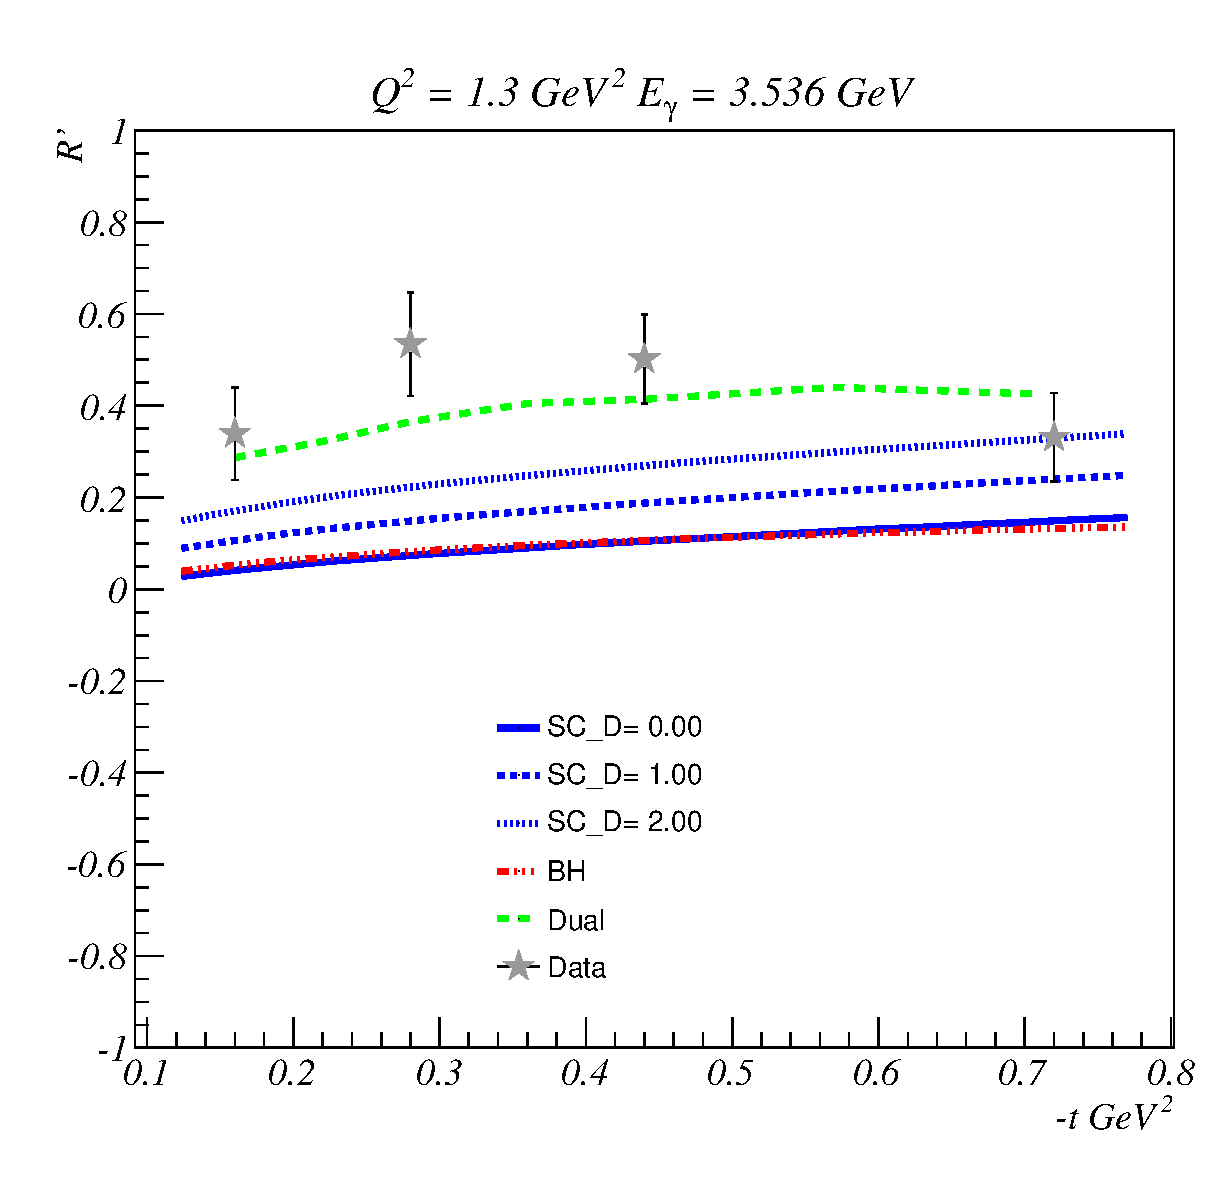
\includegraphics[scale=0.45]{R_dep_theta_var_6GeV.eps}
\caption{\small{The cosine moment of the weighted cross section, $R'$, in
the CLAS acceptance compared to GPD model calculations based on the dual
parametrization
\cite{Polyakov:2002wz,Guzey:2006xi,Guzey:2008ys,Polyakov:2008aa}
(upper, green curve), and the double distribution
\cite{Radyushkin:1998es} (lower, blue curves) for three weights applied
to the $D$-term. The BH-contribution is shown in red.}}
\label{fig:R_dep_theta_var_6GeV}
\end{figure}

Our proposed SoLID experiment builds upon experience gained from the analysis
of CLAS 6 GeV data, which has established the technique for carrying
out exclusive photoproduction experiments with quasi-real photons that we
propose for this experiment with SoLID. As will be discussed in Sec.
\ref{sec:tcs_selection}, this requires the detection of all final-state
particles except the scattered electron, for which the missing mass and
missing transverse momentum are constrained to be very small.
More specifically, this technique has also been successfully applied to pilot
measurements of timelike Compton scattering using the CLAS e1-6 and e1f data
sets. The results from this CLAS Approved Analysis (CAA-DP09-01) have been
documented in Ref.~\cite{Rafael:2010}. It demonstrated an impressive pion
pair rejection of factor of $2.07 \times 10^{-7}$. Measuring the $\phi$ cross
section in parallel with TCS showed that the flux of quasi-real photons is
well understood.
The results from the above analysis could also be compared with an TCS
analysis using the g12 data set, which was the only high-energy CLAS data set
with tagged real photons (up to 5.7 GeV) that utilized the Cherenkov counters.
These had been made ready specifically for TCS and other $e^+e^-$ physics. The
analysis of the g12 data is still ongoing, but preliminary results seems to be
in line with what was obtained with the quasi-real photon technique.
The tagged-photon beam will also make it possible to do an independent
determination of the photon flux, and offer an opportunity to explore event
topologies with only two out of the three final-state particles detected.

In addition to demonstrating the feasibility of the proposed measurement, the
pilot experiments at 6 GeV stimulated the development of new analysis methods.
An example of this was the introduction of the cosine moment $R'$, evaluated
within the acceptance of the detector in the $\varphi_{CM}-\theta_{CM}$ plane
(the lepton c.m. angles $\varphi$ and $\theta$ are defined in
Fig.~\ref{fig:Angle}). Whereas the original definition of $R$ implies using
the integration ranges shown in Eqs.(\ref{eq:S}) and (\ref{eq:R}), $R'$ adds
an function $a(\theta_{CM},\varphi_{CM})$ corresponding to the detector
acceptance for a given kinematic bin. Utilizing the same acceptance function
for both the experimental and theoretical evaluations allows a straightforward
comparison between data and predictions based on various GPD models. The
difference between $R'$ and $R$ is discussed in more detail in
Sec. \ref{sec:tcsrate} together with the projected results.

Fig.~\ref{fig:R_dep_theta_var_6GeV} shows $R'$ extracted from the combined
e1-6 and e1f data sets for four bins in $-t$, compared with two GPD model
calculations based on the dual parametrization
\cite{Polyakov:2002wz,Guzey:2006xi,Guzey:2008ys,Polyakov:2008aa} and double
distribution \cite{Radyushkin:1998es}, respectively. Results from the latter
are shown with three weights for the contribution from the $D$-term (0, 1, and
2). Both the experimental and theoretical points shown here were evaluated at
the average value for the bin, but an event-by-event approach will be adopted
in the future.

\begin{figure}[t]
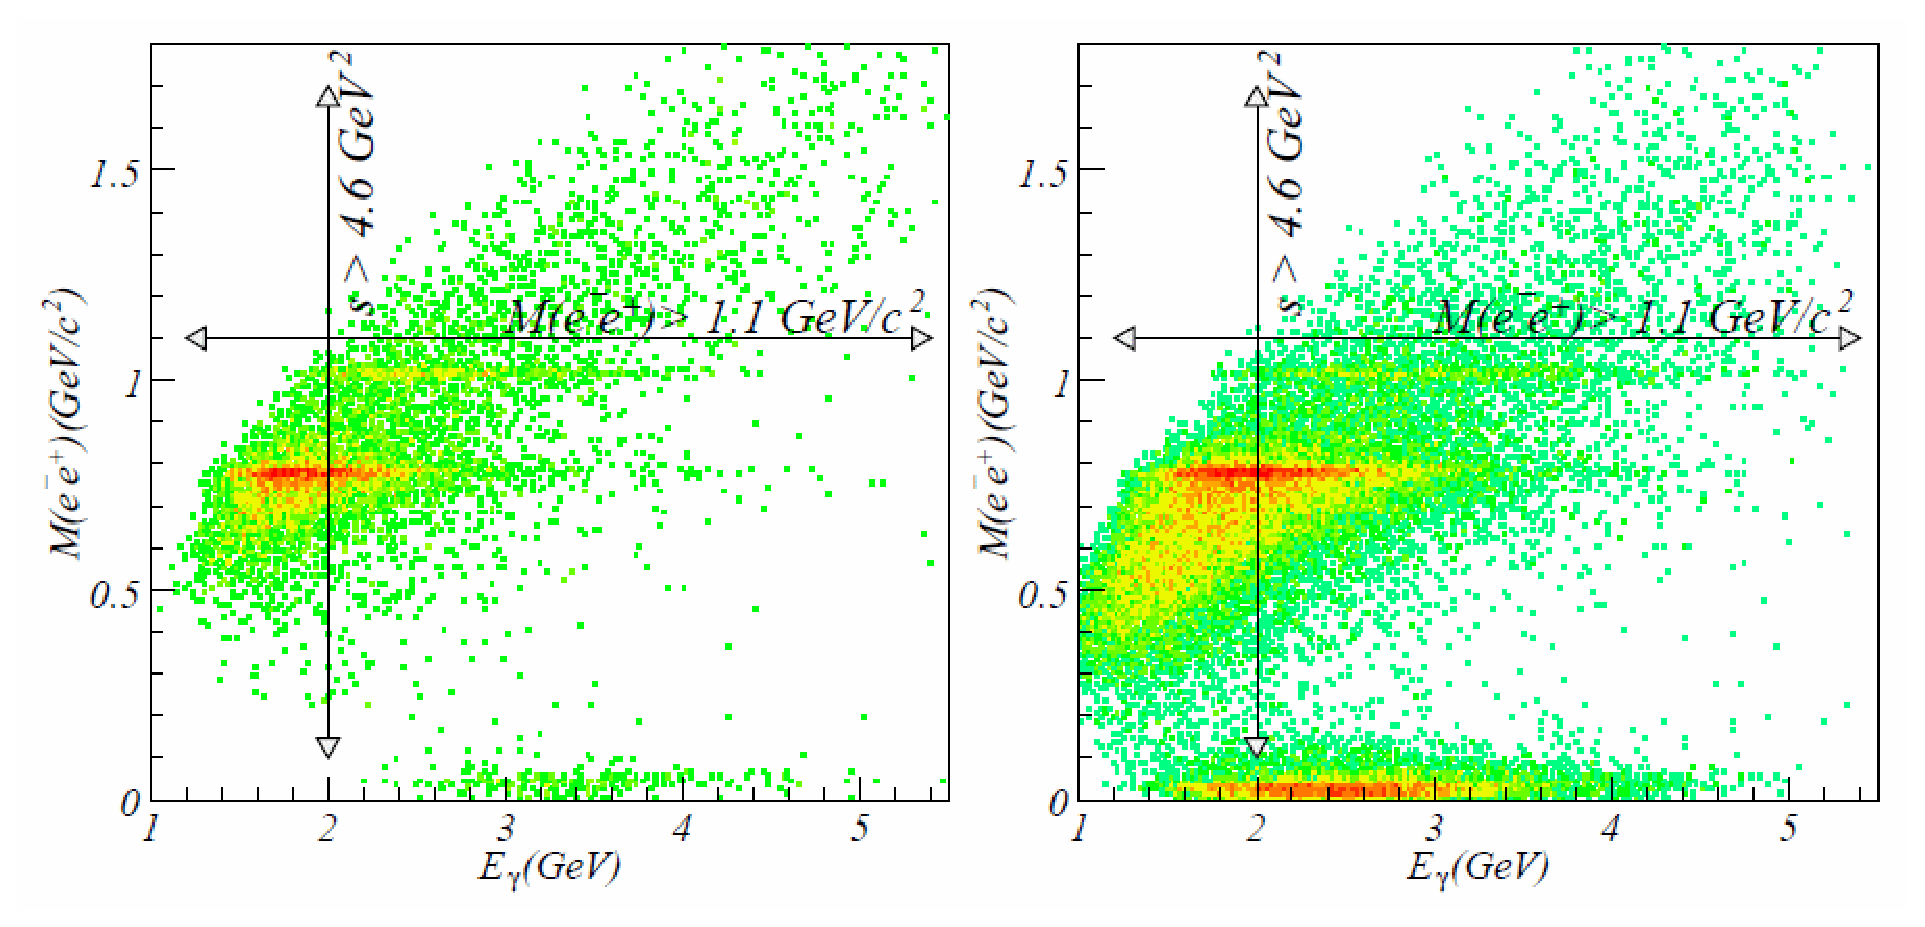
\includegraphics[scale=0.45]{TCS407.eps}
\caption{\small{$e^+e^-$ invariant mass vs. quasi-real photon energy for the
e1-6 (left) and e1f (right) data sets. Only events with $M_{ee}$ above the
$\phi$ mass were used for TCS analysis at 6 GeV.}}
\label{fig:TCS6}
\end{figure}

However, despite the usefulness of the 6 GeV data for developing the TCS
program, only the 12 GeV era will provide the required luminosity and
kinematic coverage. In particular, the higher beam energy will make it
possible to study a range of invariant lepton pair masses where there are no
meson resonances that complicate the interpretation of the measurement. As
shown in Fig.~\ref{fig:TCS6}, only data above the $\phi$ mass were used for
TCS analysis at 6 GeV, but at 12 GeV it will be possible to move this range
above the mass of the $\rho^{\prime}$.
%as shown in Fig. \ref{fig:ee_to_hadrons}.



\newpage
\section{Experimental Setup}
\label{sec:exp}
\input{tcs_experiment}

\newpage
\section{Projected Results}
\label{sec:rates}
In this section we describe the kinematics, acceptances, and projected
uncertainties. The projections have been made for 50 days of running with a
luminosity of $10^{37}$ cm$^{-2}$s$^{-1}$ on a 15 cm long liquid hydrogen
target. Only statistical uncertainties are shown. To scale to 100 days of
running, simply reduce the error bar by a factor of 0.7.

The projections are binned in three  kinematic variables: the virtuality
of the final-state photon $Q^{\prime 2} = M_{e^+e^-}^2$, the four-momentum
transfer to the nucleon $t$, and the skewness of the reaction $\eta$. The
angular distribution of the decay-lepton pair is evaluated in each bin, for
instance as a moment of the weighted cross section, using the lepton
center-of-mass angles shown in Fig.~\ref{fig:Angle}. To avoid confusion with
the lab angles, we will in this section excplicitly call these angles
$\theta_{CM}$ and $\varphi_{CM}$.


\subsection{Acceptance}
\label{sec:acc}

The selection of exclusive $e^+e^-p$ events was discussed in
Sect.~\ref{sec:tcs_selection}. Since the TCS cross section will not be
measured separately but in combination with the larger BH cross section with
which it interferes, the rate estimates for TCS were based on the BH cross
section as given in Ref.~\cite{vadim}. The resulting event distributions, 
illustrating the SoLID acceptance, are shown in Figs.~\ref{fig:t_Q2_etabin}
through \ref{fig:theta_phi_CM_Q2bin}. The first two figures show the
acceptance in six bins of $\eta$, and the last two in three bins of
$Q^{\prime 2}$. The former binning is suited for measuring the
$Q^{\prime 2}$-dependence in narrow bins of $\eta$ to study factorization
and higher-twist effects, while the latter is better for looking at the
$\eta$-dependence in wider bins of $Q^{\prime 2}$, primarily in order to
understand the impact of NLO corrections.

Fig.~\ref{fig:t_Q2_etabin} shows how the accessible range in $Q^{\prime 2}$
grows at higher values of $\eta$. It also shows how the $|t|$-coverage
shifts to higher values as $\eta$ increases.
The choice of six bins in $\eta$ is arbitrary. It is based on a desire to
to make an initial study of the $Q^{\prime 2}$-dependence in sufficiently
narrow bins in $\eta$ the interpretation will not be complicated by 
large NLO corrections. In actual  analysis, the $Q^{\prime 2}$-dependence
will also be investigated in wide $\eta$ bins. The widths of the six bins
shown have been chosen to equalize statistics in the range $0.1<\eta<0.4$
that can be covered in SoLID.
Fig.~\ref{fig:theta_phi_CM_etabin} shows the event distributions in the
$\theta_{CM}$ vs. $\varphi_{CM}$ plane for the same six bins in $\eta$.
The shape of the acceptance in the lepton CM-angles is governed by three
factors: the ``hole'' in the forward detector around the beam line, the
limit of the large-angle acceptance, and the gap between the large-angle
and forward-angle detectors in SoLID. 
The first two define the general overall shape of the distribution, while
the gap leads to a depletion of events in the middle of the band.

\begin{figure}[t]
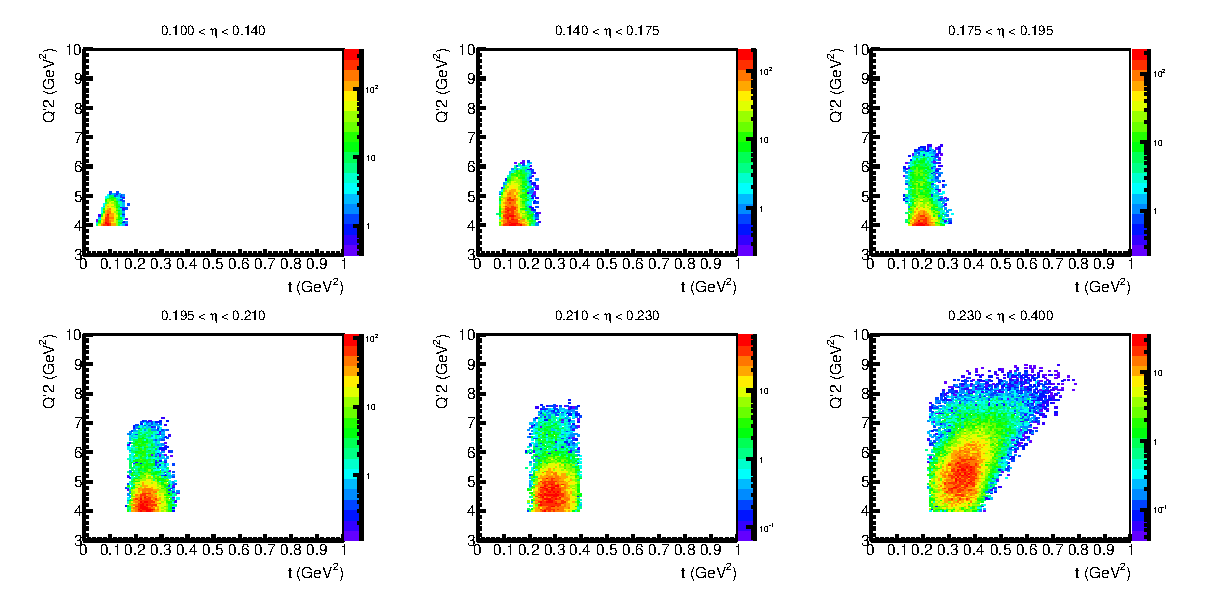
\includegraphics[scale=0.8]{t_Q2_etabin.eps}
\caption{\small{BH event distribution, in TCS kinematics, showing the SoLID
acceptance for exclusive $e^+e^-p$ production and showing the accessible
range in $Q^{\prime 2}$ and $|t|$ for six bins of $\eta$.}}
\label{fig:t_Q2_etabin}
\end{figure}

\begin{figure}[t]
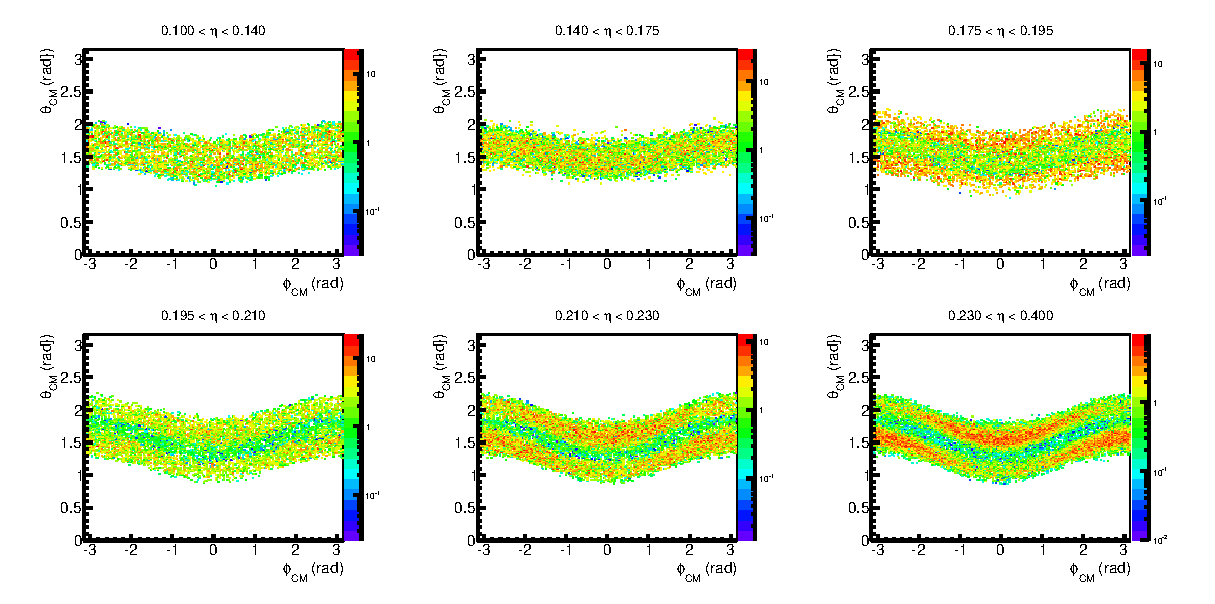
\includegraphics[scale=0.8]{theta_phi_CM_etabin.eps}
\caption{\small{BH event distribution, in TCS kinematics, showing the SoLID
acceptance for exclusive $e^+e^-p$ production and showing the accessible range
in $\theta_{CM}$ and $\varphi_{CM}$ for six bins of $\eta$.}}
\label{fig:theta_phi_CM_etabin}
\end{figure}

Once the $Q^{\prime 2}$-scaling is understood, studying the NLO corrections
through the $\eta$-dependence will not require very narrow bins in
$Q^{\prime 2}$. Fig.~\ref{fig:t_eta_Q2bin} shows the distribution of events
in $\eta$ and $|t|$ in two bins of $Q^{\prime 2}$.
Fig.~\ref{fig:theta_phi_CM_Q2bin} shows the corresponding distributions in
the $\theta_{CM}$ vs. $\varphi_{CM}$ plane.

\begin{figure}[t]
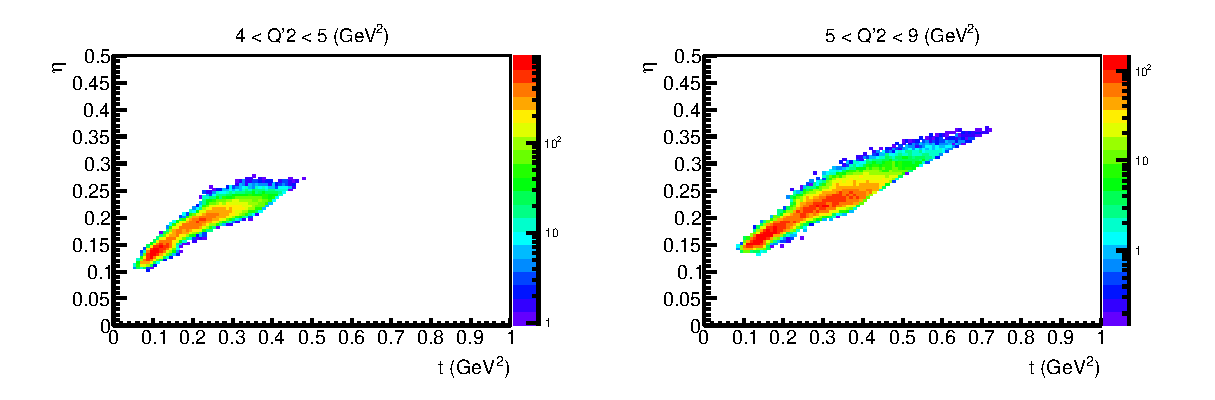
\includegraphics[scale=0.7]{t_eta_Q2bin.eps}
\caption{\small{BH event distribution, in TCS kinematics, showing the SoLID
acceptance for exclusive $e^+e^-p$ production and showing the accessible
range in $\eta$ and $|t|$ for two bins in $Q^{\prime 2}$.}}
\label{fig:t_eta_Q2bin}
\end{figure}

\begin{figure}[t]
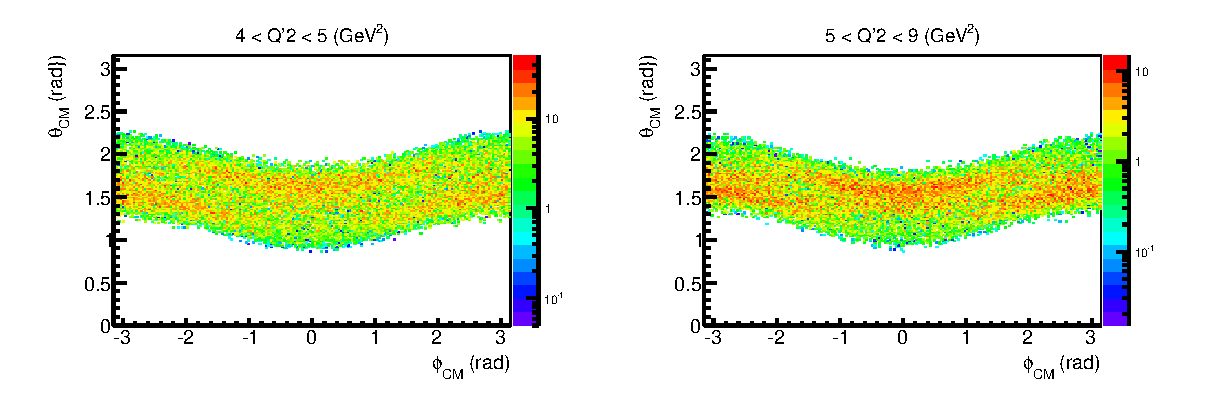
\includegraphics[scale=0.7]{theta_phi_CM_Q2bin.eps}
\caption{\small{BH event distribution, in TCS kinematics, showing the SoLID
acceptance for exclusive $e^+e^-p$ production and showing the accessible
range $\theta_{CM}$ and $\varphi_{CM}$ for tho bins of $Q^{\prime 2}$.}}
\label{fig:theta_phi_CM_Q2bin}
\end{figure}


\subsection{Projections}
\label{sec:tcsrate}

The results from the TCS analysis will come in the form of the measured
differential cross section as well as cosine and sine moments of the weighted
cross section. The cross section measurement will constrain global fits of
Compton form factors (CFFs), and could be used for extraction of helicity
amplitudes, which are related to the CFFs through Eq.~(\ref{eq:M}), by fitting
the data in the SoLID $\theta_{CM}$-$\varphi_{CM}$ acceptance.
The cosine and sine moments are also directly related to the helicity
amplitudes (and hence CFFs and GPDs). A comparison of the moments, evaluated
within the SoLID acceptance, imposes strong constraints on GPD models, and in
particular for the real part of the amplitude. 

The experimental sensitivity of the proposed measurement is easiest to
evaluate through the moments of the weighted cross section. The cosine moment
$R'$, related to $\Re e\tilde{M}^{--}$, will be used as an example. In the
extraction of the moments, the angles $\varphi_{CM}$ and $\theta_{CM}$ are
integrated over, and only the kinematic variables $Q^{\prime 2}$, $\eta$, and
$|t|$ remain.
The moment $R'$ differs from the unprimed expression defined in
Eqs.~(\ref{eq:S}) and (\ref{eq:R}) in that the latter is first integrated
over $\theta_{CM}$ and then independently over $\varphi_{CM}$, whereas the
primed moment is instead integrated over a band in the $\theta_{CM}$ vs.
$\varphi_{CM}$ plane defined through a $\varphi_{CM}$-symmetric acceptance
function $a(\theta_{CM},\varphi_{CM})$. This function is chosen such that it
coincides with the envelope of the SoLID acceptance for each bin. Using this
approach for calculating the theoretical moments allows for a direct and 
consistent comparison with the moments evaluated from the experimental data.
The absolute value of $R'$ can differ somewhat from that of $R$ due to a
non-zero BH contribution. An example of this was shown in
Fig.~\ref{fig:r_theory}. However, this does not reduce its sensitivity to
$\Re e\tilde{M}^{--}$ or GPD model predictions since the BH contribution
can be calculated exactly.
And if one wishes to do so, the difference between $R$ and $R'$ can be made
very small by adjusting the integration contour slightly, cutting away a small
fraction of events along the edges in each bin (BH can be zero even if the
contour is not a box).

Still, while the SoLID acceptance does not influence the comparison between
data and theory at the level of the contour of integration in the
$\theta_{CM}$ vs. $\varphi_{CM}$ plane, the experimental yields have to be
corrected for acceptance, primarily associated with the gap between the inner
and outer parts of the detector. This correction is done through simulations,
for which the standard SoLID package GEMC will be used. The fact that a
similar measurement will also be performed in CLAS12, where different gaps in
the acceptance are caused by the six coils of the toroidal magnet, will
greatly strengthen the confidence in the acceptance corrections and
potentially reduce the systematic uncertainties.

The projected statistical uncertainties for $R'$ are shown in
Fig.~\ref{fig:R_etabin} as a function of $Q^{\prime 2}$ for six bins in
$\eta$. The curves correspond to leading-order (LO), leading-twist
calculations using two GPD models, the dual parametrization
\cite{Polyakov:2002wz,Guzey:2006xi,Guzey:2008ys,Polyakov:2008aa} (top curve
with blue solid line) and the double distribution \cite{Radyushkin:1998es}
with $D$-term (middle curve with dash-dotted red line) and without $D$-term
(bottom curve with dashed red line). The $D$-term can also be calculated
within the framework of the dual parametrization, but it does not appear as
an independent quantity that can easily be varied, hence only one curve is
shown.
All points use 0.2 GeV$^2$ wide bins in $|t|$ close to $t=t_{min}$. This
shifts $|t|$ towards larger values in the higher $\eta$ bins, as shown in
Fig.~\ref{fig:t_Q2_etabin}.
The calculation with the dual parametrization has a proper $Q^{\prime 2}$
evolution, while the one with the double distribution only has forward
evolution, where the forward PDFs are evaluated and then ``skewed'' to
produce the GPDs at a given value of $Q^{\prime 2}$.

\begin{figure}[t]
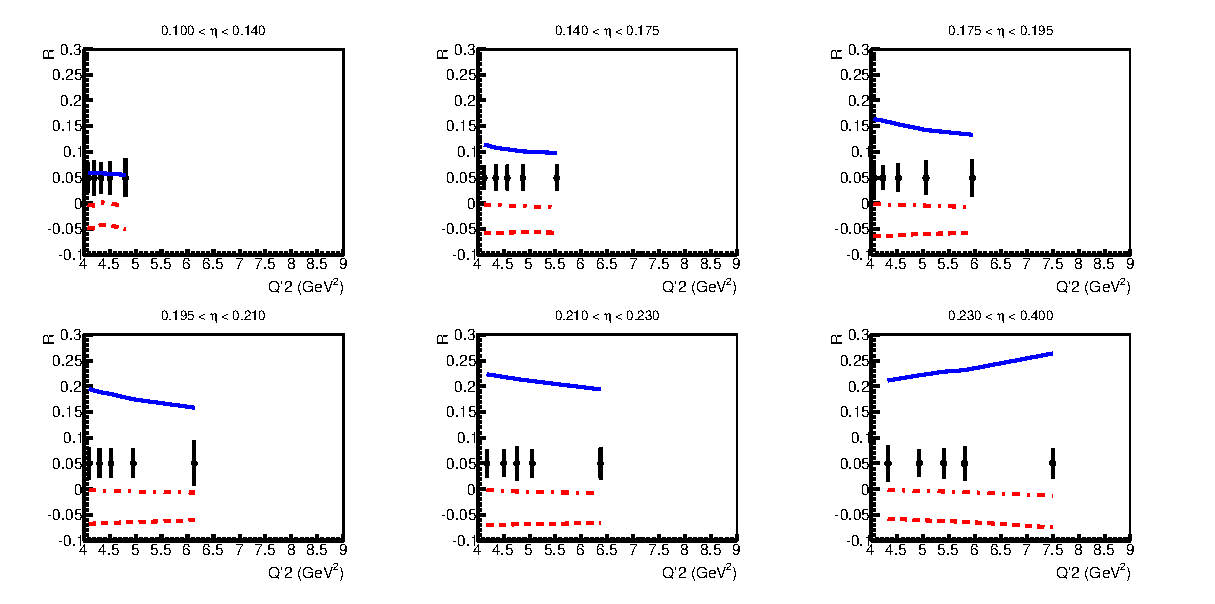
\includegraphics[scale=0.8]{R_etabin.eps}
\caption{\small{
The cosine moment of the weighted cross section, $R'$, shown as function of
$Q^{\prime 2}$ for six bins in $\eta$, in 0.2 GeV$^2$ wide bins in $|t|$
close to $t=t_{min}$. The curves correspond to leading-order, leading-twist 
calculations using two GPD models, the dual parametrization
\cite{Polyakov:2002wz,Guzey:2006xi,Guzey:2008ys,Polyakov:2008aa} (top, solid
blue curve) and the double distribution \cite{Radyushkin:1998es} with $D$-term
(middle, dash-dotted red curve) and without $D$-term (bottom, dashed red
curve). The error bars on the points correspond to 50 days of running.
The points are arbitrarily placed at $R' = 0.05$.}}
\label{fig:R_etabin}
\end{figure}

The same LO calculations can be applied to the $\eta$-dependence. The result
is shown in Fig.~\ref{fig:R_Q2bin}, where we see $R'$ as function of $\eta$
for two bins in $Q^{\prime 2}$, in 0.2 GeV$^2$ wide bins in $|t|$ close to 
$t=t_{min}$. The relation between $|t|$ and $\eta$ coverage can be seen in
Fig.~\ref{fig:t_eta_Q2bin}. As in Fig.~\ref{fig:R_etabin}, the top curve
(solid blue line) corresponds to the dual parametrization, and the middle
(dash-dotted red line) and lower (dashed red line) curves to the
double distribution with and without $D$-term, respectively. Here, the large
difference between the two models reflects the assumed dependencies of the
real part of GPD $H$ on $\tau$ (the equivalent of Bjorken $x$) that are shown
in Fig.~\ref{fig:ReImH_tau}, and to which the cosine moment $R'$ is sensitive.

\begin{figure}[t]
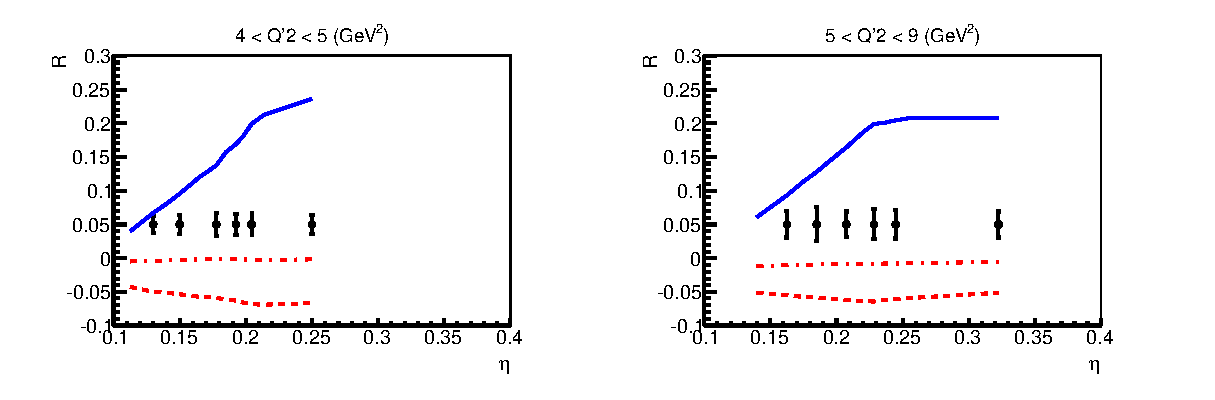
\includegraphics[scale=0.7]{R_Q2bin.eps}
\caption{\small{
The cosine moment of the weighted cross section, $R'$, shown as function of
$\eta$ for two bins in $Q^{\prime 2}$, in 0.2 GeV$^2$ wide bins in $|t|$
close to $t=t_{min}$. The curves correspond to leading-order, leading-twist
calculations using two GPD models, the dual parametrization 
\cite{Polyakov:2002wz,Guzey:2006xi,Guzey:2008ys,Polyakov:2008aa} (top, solid
blue curve) and the double distribution \cite{Radyushkin:1998es} with $D$-term
(middle, dash-dotted red curve) and without $D$-term (bottom, dashed red
curve). The error bars on the points correspond to 50 days of running.
The points are arbitrarily placed at $R' = 0.05$.}}
\label{fig:R_Q2bin}
\end{figure}

Fig.~\ref{fig:R_NLO} shows the projections based on the NLO calculations
described in Sect.~\ref{subsec:NLO}. Since the calculations in the figure
were made for $Q^{\prime 2} = 4$ GeV$^2$, the results are only shown for
one, bin in $Q^{\prime 2}$ between 4 and 6 GeV$^2$. Here, each point
corresponds to a 0.3 GeV$^2$ wide bin in $|t|$. 
The calculation was done using two GPD models: Goloskokov-Kroll (GK)
\cite{Goloskokov:2005sd,Goloskokov:2006hr,Goloskokov:2007nt,Kroll:2012sm}
and MSTW, a simple factorizing ansatz for the $t$-dependence
\cite{Berger:2001xd} with MSTW08 PDFs \cite{Martin:2009iq}.
Both LO and NLO results are shown. It is interesting to note that there is a
relatively model-independent trend in the calculations. The two upper curves
(dashed lines) are both NLO predictions, while the lower two (solid lines)
are the LO ones. It seems that for both models the NLO corrections shift
$R'$ towards more positive values, but the slope does not change much, and
hence the separation between the LO and NLO curves stays about the same for
all values of $\eta$ between 0.1 and 0.3 (going below $\eta$ of 0.1 the
separation in $R'$ does increase, but this is outside of JLab 12 GeV
kinematics). The GK model prediction (blue curves) for $R'$ is consistently
somewhat higher than MSTW (red curves) for both LO and NLO, but this
difference is small compared with the overall shift due to the NLO
corrections.
The model-independence mirrors the discussion in Sect.~\ref{subsec:NLO} where,
for instance, Fig.~\ref{fig:TCSRe2x2} suggests that the general features of
the NLO calculations do not strongly depend on the choice of model. That said,
it is worth keeping in mind that the GK model is based on $\tilde{H}$ and $H$,
while MSTW only incorporates $H$, so the predictions shown assume that other
contributions are small. It is hoped that $Q^{\prime 2}$ evolution will
be incorporated into the NLO calculation in the near future, which would
allow for reliable projections also at higher values of $Q^{\prime 2}$.

\begin{figure}[t]
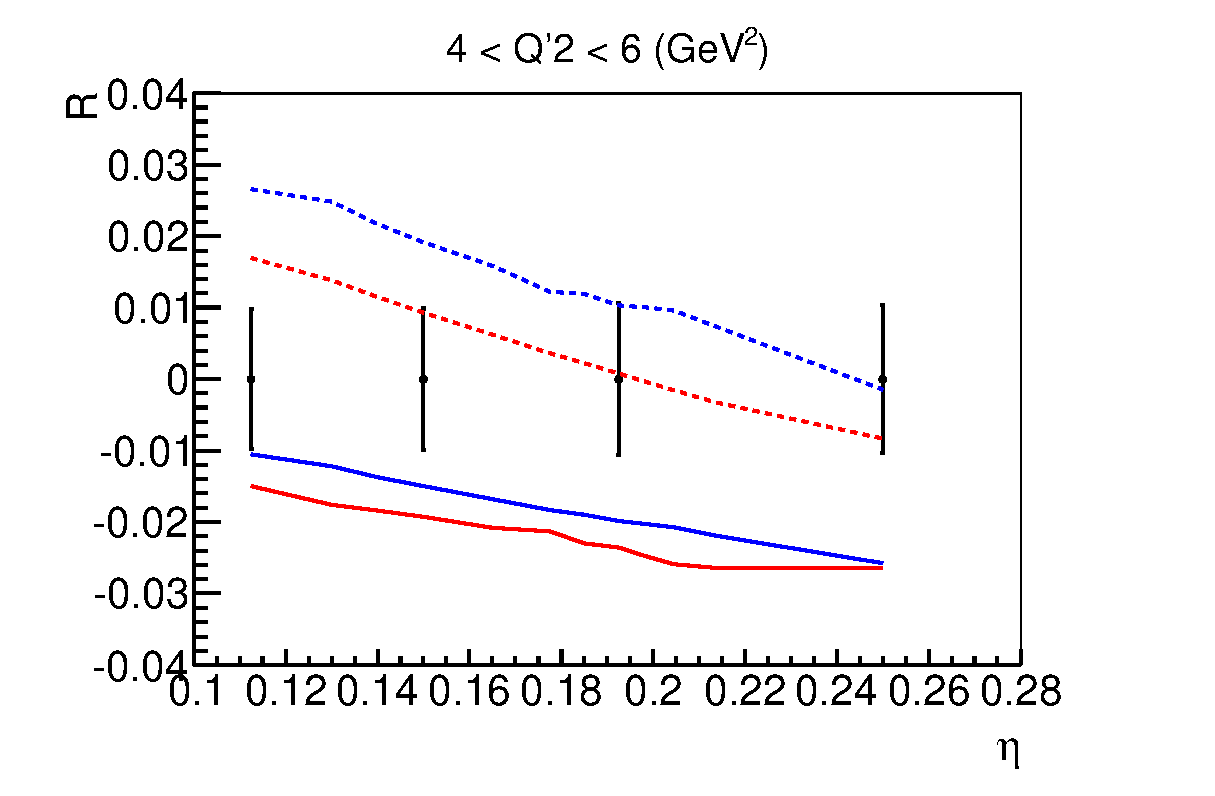
\includegraphics[scale=0.45]{R_NLO.eps}
\caption{\small{
The cosine moment of the weighted cross section, $R'$, shown as function
of $\eta$ for in a bin of $Q^{\prime 2}$ from 4 to 6 GeV$^2$ and a 0.3
GeV$^2$ wide bin of $|t|$. The upper (dotted) curves are the NLO predictions,
while the (solid) lower pair are the LO ones. Within each pair, the upper
(blue) curve was calculated using the GK model and the lower (red) one using
MSTW. The error bars on the points correspond to 50 days of running.
The points are arbitrarily placed at $R' = 0$.}}
\label{fig:R_NLO}
\end{figure}

In conclusion, the physics of deeply-virtual Compton scattering is a rich
topic, and the possibility to study the universality of GPDs and the
timelike-spacelike correspondence through TCS will add an important piece to
the puzzle. This proposed high-luminosity measurement in SoLID will make it
possible to study  the $Q^{\prime 2}$-dependence and the $\eta$-dependence.
The former will allow us to establish the scaling properties expected for
factorization, and the magnitude of our benchmark observable $R'$ will, as
shown in Fig.~\ref{fig:R_etabin}, also provide some guidance on GPD modeling.

Once the $Q^{\prime 2}$-dependence is understood, the data can be binned in
much wider bins of $Q^{\prime 2}$ for the measurement of the
$\eta$-dependence. Here, a comparison of the LO calculations for
our benchmark observable $R'$, shown in Fig.~\ref{fig:R_Q2bin}, indicates
that our sensitivity will allow us to determine whether there is a strong
$\eta$-dependence in the real part of GPD $H$ as assumed in the dual
parametrization, or if it is relatively flat as shown for the double
distribution. This alone would be a very important contribution to our
understanding of the behavior of GPDs. It is also interesting to note that LO
calculations using both the GK and MSTW models shown in Fig.~\ref{fig:R_NLO}
exhibit an $\eta$-dependence, but with a smaller and opposite slope to
that of the dual parametrization.

Measuring the $\eta$-dependence is also important for studying NLO effects.
However, in this respect it is interesting to note that our benchmark
observable $R'$ provides us with a more limited sensitivity to the NLO
corrections that one might think based on, for instance,
Fig.~\ref{fig:TCSRe2x2}. For $R'$, NLO effects create a clear shift towards
higher values, but the impact on the slope seems to be modest over the range
of $\eta$ relevant for JLab 12 GeV.
Since the NLO corrections are predominantly due to gluons, and little is
known about the gluon GPD, this scenario seems very encouraging. On one hand
it suggests that one could constrain the NLO gluonic contributions through
the magnitude of $R'$, but one the other that this would still be a good
observable for studying the behavior of quark GPDs, such as the
$\eta$-dependence of the real part of GPD $H$, even at the lower
end of the accessible $\eta$ range.
Of course, it would be even more interesting if it turned out that there were
other observables that were more sensitive to the gluons than $R'$. Then the
the lower part of the $\eta$ range covered by this proposed TCS experiment
could, perhaps in conjunction with vector meson production, provide a novel
approach for probing the glue in the valence region.


\newpage
\section{Systematic Uncertainties}
\label{sec:systematics}
The two main sources of systematic uncertainty for the proposed measurement
are acceptance corrections and lepton identification. The former can be
expected to comparable to estimates for cross section measurements with
CLAS12, \textit{i.e.}, to be at least of the order of 5\%. As discussed in
Sec.~\ref{sec:acc}, the acceptance studies will be performed through GEMC
simulations -- the standard GEANT4 package for SoLID.

As described in Sec.~\ref{sec:tcs_selection}, lepton identification will be
performed using the Cherenkov counters (CC) and the electromagnetic
calorimeters (EC). All events used for the analysis of this proposed
experiment will have both leptons detected in one of the ECs, and at least
within the (angular and momentum) acceptance of the CCs. For those pairs, the
two-pion rejection factor is expected to be at about $10^7$. The
remaining pairs will be discarded from the analysis. This will not have any
significant impact on the statistical uncertainty.

In the photon-energy range of the proposed experiment, the total cross section
for $\pi^+\pi^-$ production is 0.1 mb. With a pion pair rejection factor of
$10^7$, there would be a pion background at the 5\% level if the
total $e^+e^-$ cross section was 0.1 nb. This is comparable to the $J/\psi$
cross section in JLab 12 GeV kinematics. The BH cross section integrated over
$0.5 < Q^{\prime 2} < 7$ GeV$^2$ at $E_\gamma = 11$ GeV is 34 nb. For most
kinematics, and in particular those in the primary range of interest
(\textit{i.e.}, for $4 < Q^{\prime 2} < 9$ GeV$^2$), the contribution to the
total uncertainty from lepton pair misidentification should be small compared
with the statistical uncertainty, and the systematic uncertainty in the
acceptance correction. Performing the measurement with two independent setups,
SoLID and CLAS12, will greatly increase our confidence in being able to
correctly estimate the systematic uncertainties, and in particular those
related to acceptance.


\newpage
\section{Beam Time}
\label{sec:beamtime}
This proposed experiment will require a longitudinally polarized ($>80$\%) 11
GeV beam and an unpolarized proton target in the SoLID detector.
For photoproduction using quasi-real photons, the detector will need a recoil
baryon detection and identification capability. This could be most easily
accomplished by extending the high-resolution time-of-flight system to cover
the same angular range as the calorimeter.
Furthermore, specifically for $e^+e^-$ photoproduction, the trigger has to be
set up for a coincidence of two leptons, with the additional condition that
at least one of them produces a signal in the Cherenkov. Events where both
leptons hit the outer part of the calorimeter where there is no Cherenkov
coverage would not be useful for offline analysis due to the low pion pair
suppression factor. If it would desirable to reduce the trigger rate further,
a condition of a third particle could be added, even though this would make
it more difficult to evaluate the trigger efficiency. Alternatively, a more
open trigger satisfying the conditions above would also be a good solution.
With the provisions above, the beam-time can, in part or in full, be shared
with already approved experiments, such as E12-12-006~\cite{E12-12-006}.


 
\clearpage
%\bibliographystyle{h-physrev}
\bibliographystyle{hunsrt}
%\bibliographystyle{unsrt}
\bibliography{tcs_refs}

\end{document}
